


\documentclass[a4paper]{article}\usepackage[]{graphicx}\usepackage[]{color}
%% maxwidth is the original width if it is less than linewidth
%% otherwise use linewidth (to make sure the graphics do not exceed the margin)
\makeatletter
\def\maxwidth{ %
  \ifdim\Gin@nat@width>\linewidth
    \linewidth
  \else
    \Gin@nat@width
  \fi
}
\makeatother

\definecolor{fgcolor}{rgb}{0.345, 0.345, 0.345}
\newcommand{\hlnum}[1]{\textcolor[rgb]{0.686,0.059,0.569}{#1}}%
\newcommand{\hlstr}[1]{\textcolor[rgb]{0.192,0.494,0.8}{#1}}%
\newcommand{\hlcom}[1]{\textcolor[rgb]{0.678,0.584,0.686}{\textit{#1}}}%
\newcommand{\hlopt}[1]{\textcolor[rgb]{0,0,0}{#1}}%
\newcommand{\hlstd}[1]{\textcolor[rgb]{0.345,0.345,0.345}{#1}}%
\newcommand{\hlkwa}[1]{\textcolor[rgb]{0.161,0.373,0.58}{\textbf{#1}}}%
\newcommand{\hlkwb}[1]{\textcolor[rgb]{0.69,0.353,0.396}{#1}}%
\newcommand{\hlkwc}[1]{\textcolor[rgb]{0.333,0.667,0.333}{#1}}%
\newcommand{\hlkwd}[1]{\textcolor[rgb]{0.737,0.353,0.396}{\textbf{#1}}}%

\usepackage{framed}
\makeatletter
\newenvironment{kframe}{%
 \def\at@end@of@kframe{}%
 \ifinner\ifhmode%
  \def\at@end@of@kframe{\end{minipage}}%
  \begin{minipage}{\columnwidth}%
 \fi\fi%
 \def\FrameCommand##1{\hskip\@totalleftmargin \hskip-\fboxsep
 \colorbox{shadecolor}{##1}\hskip-\fboxsep
     % There is no \\@totalrightmargin, so:
     \hskip-\linewidth \hskip-\@totalleftmargin \hskip\columnwidth}%
 \MakeFramed {\advance\hsize-\width
   \@totalleftmargin\z@ \linewidth\hsize
   \@setminipage}}%
 {\par\unskip\endMakeFramed%
 \at@end@of@kframe}
\makeatother

\definecolor{shadecolor}{rgb}{.97, .97, .97}
\definecolor{messagecolor}{rgb}{0, 0, 0}
\definecolor{warningcolor}{rgb}{1, 0, 1}
\definecolor{errorcolor}{rgb}{1, 0, 0}
\newenvironment{knitrout}{}{} % an empty environment to be redefined in TeX

\usepackage{alltt}

\usepackage{hyperref}
\usepackage{graphicx}
\usepackage{longtable}
\usepackage[utf8]{inputenc}
\usepackage[spanish]{babel}
\usepackage{underscore}

\newcommand{\etal}{{\it et alt.}}
\newcommand{\R}{{\it R}}
\newcommand{\Rpackage}[1]{{\texttt{#1}}}
\newcommand{\Rcode}[1]{{\texttt{#1}}}
\newcommand{\Rfun}[1]{{\texttt{#1}}}

\title{Genómica funcional y análisis de microarrays\\
  Primera PEC : Selección de genes expresados diferencialmente}

\author{Alex Sánchez}

\bibliographystyle{plain}
\IfFileExists{upquote.sty}{\usepackage{upquote}}{}
\begin{document}

\setkeys{Gin}{width=0.7\textwidth} % Sets default width for R-Sweave generated figures

\maketitle

\tableofcontents

\section{Introducción y objetivos}

Este documento presenta una solución al ejercicio de análisis de microarrays propuesto en la asignatura de \emph{Genómica Funcional y Análisis de Microarrays}. Su objetivo no es mostrar como realizar el mejor análisis de microarrays posible sino como hacerlo utilizando los conceptos y ejemplos proporcionados en las unidades dedicadas a este tema.

\subsection{Estructura del documento}

Típicamente un trabajo científico o técnico se organiza en varias partes: \emph{Introducción}, \emph{Material y Métodos}, \emph{Resultados} y \emph{Discusión}. Dado que el objetivo de este estudio es demostrar la aplicación de los métodos de análisis explicados en la asignatura esta estructura se relajará. Después de la introducción se realizará una breve descripción del proceso general y los métodos utilizados en cada paso. A continuación se presentarán los resultados obtenidos en cada fase del análisis. Finalmente se presentará una breve discusión sobre las posibles limitaciones encontradas.

\subsection{Objetivos}

El objetivo de este trabajo es realizar un análisis de datos de microarrays 
para encontrar genes diferencialmente expresados entre varios tipos de tumores de cancer de mama clasificados en tres grupos: apocrinos (APO), basales (BAS) y luminales (LUMI). 

Esta clasificación se basa en la resistencia de los tumores a los receptores de estrógenos y de andrógenos. 
\begin{itemize}
\item Los tumores clasificados como ``APO'' son negativos para los receptores de estrógenos (ER-) y positivos para los receptores de andrógenos (AR+).
\item  los clasificados como ``LUMI'' son (ER+) y (AR+) y
\item los clasificados como ``BAS'' son (ER-) y (AR-).
\end{itemize}

Es conveniente destacar que, de hecho, el objetivo de la práctica difiere del objetivo del artículo en que se basa. Mientras que el artículo se busca  \emph{descubrir} los tres grupos con los que trabajamos en este ejercicio se pretende caracterizarlos a través de los gene que se expresan de forma distinta entre ellos. No deja de ser un problema del tipo ``el huevo y la gallina'', es decir: \emph{¿Puesto que se trata de grupos distintos encontramos genes que se expresan diferencialmente entre ellos o dado que hay genes que se expresan diferencialmente podemos deducir que son grupos distintos?}

\section{Materiales y métodos}

\subsection{Etapas del analisis}

El análisis se ha realizado siguiendo las pautas descritas en los capítulos 6 a 11 de los apuntes de la asignatura \url{http://ueb.vhir.org/cursos/Microarrays} y resumidos en la figura \ref{fig:pipeline}.

\begin{figure}[htbp]\begin{center}
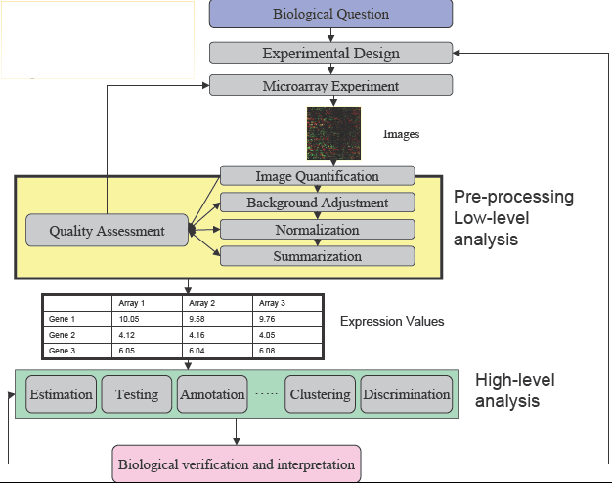
\includegraphics[width=9cm]{images/analysisProcess}\\
\caption{The Microarray Analysis Process}\label{fig:pipeline}
\end{center}
\end{figure}

\subsection{Métodos de análisis}

Antes de hibridar los microarrays\footnote{Esta primera parte es ficticia en tanto que no hemos tendio acceso al proceso de elaboración de los microarrays, por lo que he escrito lo que suele ponerse en esta parte} se comprobó la calidad del cRNA de cada muestra. Sólo las que demostraron una calidad suficiente --presumiblemente un valor de ``Bio-analyser''\footnote{Sistema para el análisi de la calidad del RNA} igual o superior a 7-- se sometieron a análisis posterior.. 

Los valores ``crudos'' de expresión obtenidos directamente de los archivos CEL se preprocesa utilizando el método de RMA (\cite{Irizarry:2003}), un proceso de tres pasos que integra la corrección de fondo, la normalización y el resumen de los valores del grupo de sondas en un único valor de expresión ``absoluta''. Dichos valores normalizados fueron la base para todos los análisis.

Antes de la selección de genes los valores normalizados se sometieron a un filtraje no específico para eliminar los genes de baja 
%señal (los genes cuya media de la señal en cada grupo no supera un umbral mínimo) y los genes de baja 
variabilidad (los genes cuyo rango intercuartil entre todas las muestras no superó un umbral mínimo).

La selección de genes diferencialmente expresados entre condiciones experimentales se basó en el método desarrollado por Smyth y otros ~\cite{Smyth:2004}.

%La selecci\'on de genes ​diferencialmente expresados entre condiciones experimentales se bas\'o en la utilización de modelos lineales complementados con una moderación de la varianza mediante m\'etodos bayesianos emp\'iricos siguiendo la metodolog\'ia desarrollada por Smyth \cite{Smyth:2004}.

Este método extiende el análisis de la varianza clásico utilizando métodos Bayesianos empíricos para combinar la información de cada gen individual con la de todos los genes restantes para obtener mejores estimaciones de error. Esto es de gran utilidad en análisis de microarrays, un contexto en el que el tamaño de las muestras es a menudo pequeño lo que puede dar lugar a estimaciones de los errores erráticos y, en consecuencia, p--valores que no son de fiar.

Los genes más relevantes de cada comparación se resaltaron utilizando ``volcano-plots'', 
que organizan los genes a lo largo de dos dimensiones que podemos considerar de importancia biológica y estadística. El eje horizontal representa el cambio medio de expresión entre los dos grupos (en una escala logarítmica, por lo que la regulación hacia arriba y abajo aparecen simétrica), y el segundo (vertical) representa el ``menos logaritmo del p-valor'' por lo que los genes cuyo p-valor asociado sea inferior aparecen más arriba. El primer eje indica el impacto biológico del cambio, y el segundo indica la evidencia estadística, o la fiabilidad de dicho cambio.


Con el fin de hacer frente a la problemática derivada del hecho de que muchas pruebas (una por cada gen) se realizan simultáneamente, se realizo un ajuste de p--valores para obtener control sobre la tasa de falsos positivos usando el método de Benjamini y Hochberg (\cite{BenjaminiHochberg:1995}).



Los genes seleccionados como diferencialmente expresados se agruparon para buscar patrones comunes de expresión entre condiciones experimentales.
Para ello se utilizaron mapas de colores o ``Heatmaps'' que realizan una agrupación jerárquica de los genes y/o las muestras y la representan mediante una gama de colores apropiada, de forma que valores altos o bajos se corresponden a colores distintos de la gama escogida.

Las listas de genes diferencialmente expresados se anotaron en diversas bases de datos (Entrez, Unigene, Gene Ontology, KEGG, ...) utilizando los paquetes de anotación para microarrays de affymetrix disponibles en el proyecto Bioconductor (\url{http://bioconductor.org}).

Para contribuir a la interpretación biológica de los resultados se realizó un análisis de enriquecimiento \cite{Gentleman:2004, Falcon:2007} que busca establecer si las categorias funcionales de los genes seleccionados aparecen entre estos genes con mayor (o menor) frecuencia que entre todos los del genoma. De ser así se indica que la lista de genes se encuentra ``enriquecida'' en estas funcionalidades, o lo que es lo mismo que los procesos afectados por las diferencias son éstos.

\subsubsection{Herramientas y procedimientos  bioinformáticos de análisis}

Los análisis estadísticos se realizaron utilizando el lenguaje estadístico  \R  y las librerías  desarrolladas para el análisis de microarray en el proyecto de Bioconductor (\url{www.bioconductor.org}). Para más detalle sobre los métodos descritos en esta sección puede consultarse \cite{Gentleman:2005}.

El código siguiente se utilizó para instalar los paquetes de Bioconductor necesarios para el análisis.

\begin{knitrout}
\definecolor{shadecolor}{rgb}{0.969, 0.969, 0.969}\color{fgcolor}\begin{kframe}
\begin{alltt}
\hlstd{installifnot} \hlkwb{<-} \hlkwa{function} \hlstd{(}\hlkwc{pckgName}\hlstd{)\{}
  \hlkwa{if}\hlstd{(}\hlopt{!}\hlstd{(}\hlkwd{require}\hlstd{(pckgName,} \hlkwc{character.only}\hlstd{=}\hlnum{TRUE}\hlstd{)))\{}
    \hlkwd{source}\hlstd{(}\hlstr{"http://Bioconductor.org/biocLite.R"}\hlstd{)}
    \hlkwd{biocLite}\hlstd{(pckgName)}
  \hlstd{\}}
\hlstd{\}}
\hlkwd{installifnot}\hlstd{(}\hlstr{"Biobase"}\hlstd{)}
\end{alltt}


{\ttfamily\noindent\itshape\color{messagecolor}{\#\# Loading required package: Biobase\\\#\# Loading required package: BiocGenerics\\\#\# Loading required package: parallel\\\#\# \\\#\# Attaching package: 'BiocGenerics'\\\#\# \\\#\# The following objects are masked from 'package:parallel':\\\#\# \\\#\#\ \ \ \  clusterApply, clusterApplyLB, clusterCall, clusterEvalQ,\\\#\#\ \ \ \  clusterExport, clusterMap, parApply, parCapply, parLapply,\\\#\#\ \ \ \  parLapplyLB, parRapply, parSapply, parSapplyLB\\\#\# \\\#\# The following object is masked from 'package:stats':\\\#\# \\\#\#\ \ \ \  xtabs\\\#\# \\\#\# The following objects are masked from 'package:base':\\\#\# \\\#\#\ \ \ \  anyDuplicated, append, as.data.frame, as.vector, cbind,\\\#\#\ \ \ \  colnames, do.call, duplicated, eval, evalq, Filter, Find, get,\\\#\#\ \ \ \  intersect, is.unsorted, lapply, Map, mapply, match, mget,\\\#\#\ \ \ \  order, paste, pmax, pmax.int, pmin, pmin.int, Position, rank,\\\#\#\ \ \ \  rbind, Reduce, rep.int, rownames, sapply, setdiff, sort,\\\#\#\ \ \ \  table, tapply, union, unique, unlist, unsplit\\\#\# \\\#\# Welcome to Bioconductor\\\#\# \\\#\#\ \ \ \  Vignettes contain introductory material; view with\\\#\#\ \ \ \  'browseVignettes()'. To cite Bioconductor, see\\\#\#\ \ \ \  'citation("{}Biobase"{})', and for packages 'citation("{}pkgname"{})'.}}\begin{alltt}
\hlkwd{installifnot}\hlstd{(}\hlstr{"hgu133a.db"}\hlstd{)}
\end{alltt}


{\ttfamily\noindent\itshape\color{messagecolor}{\#\# Loading required package: hgu133a.db\\\#\# Loading required package: AnnotationDbi\\\#\# Loading required package: stats4\\\#\# Loading required package: GenomeInfoDb\\\#\# Loading required package: S4Vectors\\\#\# Creating a generic function for 'nchar' from package 'base' in package 'S4Vectors'\\\#\# Loading required package: IRanges\\\#\# Loading required package: org.Hs.eg.db\\\#\# Loading required package: DBI}}\begin{alltt}
\hlkwd{installifnot}\hlstd{(}\hlstr{"affy"}\hlstd{)}
\end{alltt}


{\ttfamily\noindent\itshape\color{messagecolor}{\#\# Loading required package: affy}}\begin{alltt}
\hlkwd{installifnot}\hlstd{(}\hlstr{"affyPLM"}\hlstd{)}
\end{alltt}


{\ttfamily\noindent\itshape\color{messagecolor}{\#\# Loading required package: affyPLM\\\#\# Loading required package: gcrma\\\#\# Loading required package: preprocessCore}}\begin{alltt}
\hlkwd{installifnot}\hlstd{(}\hlstr{"arrayQualityMetrics"}\hlstd{)}
\end{alltt}


{\ttfamily\noindent\itshape\color{messagecolor}{\#\# Loading required package: arrayQualityMetrics}}

{\ttfamily\noindent\color{warningcolor}{\#\# Warning: replacing previous import by 'ggplot2::unit' when loading 'Hmisc'}}

{\ttfamily\noindent\color{warningcolor}{\#\# Warning: replacing previous import by 'ggplot2::arrow' when loading 'Hmisc'}}

{\ttfamily\noindent\color{warningcolor}{\#\# Warning: replacing previous import by 'scales::alpha' when loading 'Hmisc'}}\begin{alltt}
\hlkwd{installifnot}\hlstd{(}\hlstr{"genefilter"}\hlstd{)}
\end{alltt}


{\ttfamily\noindent\itshape\color{messagecolor}{\#\# Loading required package: genefilter\\\#\# \\\#\# Attaching package: 'genefilter'\\\#\# \\\#\# The following object is masked from 'package:base':\\\#\# \\\#\#\ \ \ \  anyNA}}\begin{alltt}
\hlkwd{installifnot}\hlstd{(}\hlstr{"limma"}\hlstd{)}
\end{alltt}


{\ttfamily\noindent\itshape\color{messagecolor}{\#\# Loading required package: limma\\\#\# \\\#\# Attaching package: 'limma'\\\#\# \\\#\# The following object is masked from 'package:BiocGenerics':\\\#\# \\\#\#\ \ \ \  plotMA}}\begin{alltt}
\hlkwd{installifnot}\hlstd{(}\hlstr{"hgu133a.db"}\hlstd{)}
\hlkwd{installifnot}\hlstd{(}\hlstr{"annotate"}\hlstd{)}
\end{alltt}


{\ttfamily\noindent\itshape\color{messagecolor}{\#\# Loading required package: annotate\\\#\# Loading required package: XML}}\begin{alltt}
\hlkwd{installifnot}\hlstd{(}\hlstr{"annaffy"}\hlstd{)}
\end{alltt}


{\ttfamily\noindent\itshape\color{messagecolor}{\#\# Loading required package: annaffy\\\#\# Loading required package: GO.db\\\#\# \\\#\# Loading required package: KEGG.db\\\#\# \\\#\# KEGG.db contains mappings based on older data because the original\\\#\#\ \  resource was removed from the the public domain before the most\\\#\#\ \  recent update was produced. This package should now be\\\#\#\ \  considered deprecated and future versions of Bioconductor may\\\#\#\ \  not have it available.\ \ Users who want more current data are\\\#\#\ \  encouraged to look at the KEGGREST or reactome.db packages}}\begin{alltt}
\hlkwd{installifnot}\hlstd{(}\hlstr{"hwriter"}\hlstd{)}
\end{alltt}


{\ttfamily\noindent\itshape\color{messagecolor}{\#\# Loading required package: hwriter}}\begin{alltt}
\hlkwd{installifnot}\hlstd{(}\hlstr{"gplots"}\hlstd{)}
\end{alltt}


{\ttfamily\noindent\itshape\color{messagecolor}{\#\# Loading required package: gplots\\\#\# \\\#\# Attaching package: 'gplots'\\\#\# \\\#\# The following object is masked from 'package:IRanges':\\\#\# \\\#\#\ \ \ \  space\\\#\# \\\#\# The following object is masked from 'package:stats':\\\#\# \\\#\#\ \ \ \  lowess}}\begin{alltt}
\hlkwd{installifnot}\hlstd{(}\hlstr{"GOstats"}\hlstd{)}
\end{alltt}


{\ttfamily\noindent\itshape\color{messagecolor}{\#\# Loading required package: GOstats\\\#\# Loading required package: Category\\\#\# Loading required package: Matrix\\\#\# \\\#\# Attaching package: 'Matrix'\\\#\# \\\#\# The following object is masked from 'package:IRanges':\\\#\# \\\#\#\ \ \ \  expand\\\#\# \\\#\# Loading required package: graph\\\#\# \\\#\# Attaching package: 'graph'\\\#\# \\\#\# The following object is masked from 'package:XML':\\\#\# \\\#\#\ \ \ \  addNode\\\#\# \\\#\# \\\#\# Attaching package: 'GOstats'\\\#\# \\\#\# The following object is masked from 'package:AnnotationDbi':\\\#\# \\\#\#\ \ \ \  makeGOGraph}}\end{kframe}
\end{knitrout}



\section{Obtención y lectura de los datos}

\subsection{Los datos para el análisis}

Los datos en que se basa el estudio se han obtenido a partir de tumores de mama (``advanced/inflammatory breast tumours'') y fueron tomados antes del tratamiento de pacientes enrolados en un estudio clínico (EORTC 10994). 

Los microarrays se prepararon a partir de RNA total extraído de secciones de 25 mm de biopsias y amplificados mediante el procedimiento ``Eberwine T7 procedure'' siguiendo el protocolo indicado por Affymetrix para pequeñas muestras.

Los datos de los microarrays se encuentran en Gene Expression Omnibus (GEO) con el número de serie GSE1561. Puede accederse a ellos  en el siguiente enlace \url{http://www.ncbi.nlm.nih.gov/geo/query/acc.cgi?acc=GSE1561}. El artículo de Farmer (\cite{Farmer2005}) \etal (\url{http://www.ncbi.nlm.nih.gov/pubmed/15897907}) describe el estudio.

\subsubsection{Localización de los datos }

Como es habitual en este curso supondremos que trabajamos en un directorio 
escogido por nosotros y cuya localización se asigna a la variable \texttt{workingDir}.

Asumiremos que los datos se encuentran en un subdirectorio del anterior, denominado ``data'' que se almacenará en la variable \texttt{dataDir} y que los resultados se almacenarán en un directorio ``results'' cuyo nombre completo se almacenará en la variable  \texttt{resultsDir}.

\begin{knitrout}
\definecolor{shadecolor}{rgb}{0.969, 0.969, 0.969}\color{fgcolor}\begin{kframe}
\begin{alltt}
\hlstd{workingDir} \hlkwb{<-}\hlkwd{getwd}\hlstd{()}
\hlstd{dataDir} \hlkwb{<-}\hlkwd{file.path}\hlstd{(workingDir,} \hlstr{"data"}\hlstd{)}
\hlstd{resultsDir} \hlkwb{<-} \hlkwd{file.path}\hlstd{(workingDir,}\hlstr{"results"}\hlstd{)}
\hlstd{celfilesDir} \hlkwb{<-} \hlkwd{file.path}\hlstd{(workingDir,}\hlstr{"celfiles"}\hlstd{)}
\hlkwd{setwd}\hlstd{(workingDir)}
\end{alltt}
\end{kframe}
\end{knitrout}

\subsubsection{Selección de muestras para el análisis}

Este análisis se ha basado en un subconjunto de muestras del estudio original.
Las muestras se han obtenido de la lista original mediante un pequeño script de \R.

De la dirección  \url{http://www.ncbi.nlm.nih.gov/geo/query/acc.cgi?acc=GSE1561}  es posible descargar un archivo comprimido con los 49 archivos ``.cel''. Con el fin de simplificar el análisis se decidió seleccionar aleatoriamente 5 arrays de cada grupo utilizando a partir de la información contenida en el archivo: ``Asignacion_de_Muestras_A_Grupos.csv'' elaborado a partir de la información sobre el diseño experimental contenida en: \url{http://www.ncbi.nlm.nih.gov/geo/gds/profileGraph.cgi?gds=1329}

\begin{knitrout}
\definecolor{shadecolor}{rgb}{0.969, 0.969, 0.969}\color{fgcolor}\begin{kframe}
\begin{alltt}
\hlstd{muestras} \hlkwb{<-} \hlkwd{read.csv2}\hlstd{(}\hlkwd{file.path}\hlstd{(dataDir,} \hlstr{"Asignacion_de_muestras_a_grupos.csv"}\hlstd{),}
                      \hlkwc{head}\hlstd{=T)}
\hlstd{misMuestras} \hlkwb{<-} \hlkwd{as.character} \hlstd{(muestras}\hlopt{$}\hlstd{Sample)}
\hlstd{paraAnalisis} \hlkwb{<-} \hlkwd{c}\hlstd{(}\hlkwd{sample}\hlstd{(misMuestras[}\hlnum{1}\hlopt{:}\hlnum{6}\hlstd{],} \hlnum{5}\hlstd{),}
                  \hlkwd{sample}\hlstd{(misMuestras[}\hlnum{7}\hlopt{:}\hlnum{20}\hlstd{],} \hlnum{5}\hlstd{),}
                  \hlkwd{sample}\hlstd{(misMuestras[}\hlnum{23}\hlopt{:}\hlnum{48}\hlstd{],} \hlnum{5}\hlstd{))}
\hlstd{alAnalisis} \hlkwb{<-}\hlstd{muestras[muestras}\hlopt{$}\hlstd{Sample} \hlopt \hlstd{paraAnalisis,]}
\hlkwd{write.table}\hlstd{(alAnalisis,} \hlkwc{file}\hlstd{=}\hlkwd{file.path}\hlstd{(dataDir,} \hlstr{"targets.txt"}\hlstd{),}
            \hlkwc{sep}\hlstd{=}\hlstr{"\textbackslash{}t"}\hlstd{,} \hlkwc{row.names}\hlstd{=}\hlnum{FALSE}\hlstd{,} \hlkwc{quote}\hlstd{=}\hlnum{FALSE}\hlstd{)}
\end{alltt}
\end{kframe}
\end{knitrout}

\subsubsection{Lectura de los datos}

La lectura de datos se lleva a cabo utilizando las clases y métodos definidas en los paquetes \Rcode{Biobase} y \Rcode{affy} de Bioconductor.

Una forma cómoda de leer los datos y, al mismo tiempo, asignar a cada muestra los valores de las covariables (por ejemplo el grupo para el analisis) consiste en crear un pequeño archivo de texto, que suele denominarse \Rcode{targets.txt} y que contiene la identificacion de cada archivo con la asignación de cada muestra a cada condición experimental. El archivo targets para este caso tiene el aspecto que se muestra en la tabla \ref{table.targets}.

\begin{kframe}


{\ttfamily\noindent\itshape\color{messagecolor}{\#\# Loading required package: xtable}}\end{kframe}% latex table generated in R 3.2.2 by xtable 1.7-4 package
% Sun Jan 10 17:23:31 2016
\begin{longtable}{rllll}
  \hline
 & Sample & Ids & SampleIDs & Group \\ 
  \hline
GSM26878.CEL & GSM26878 & PF14 EnPnT2N1G2 & PF14 & A \\ 
  GSM26883.CEL & GSM26883 & PF19 EnPuT4N0Gu & PF19 & A \\ 
  GSM26887.CEL & GSM26887 & PF23 EnPnT2N0G2 & PF23 & A \\ 
  GSM26903.CEL & GSM26903 & PF39 EnPuT4N0Gu & PF39 & A \\ 
  GSM26910.CEL & GSM26910 & PF46 EnPnT4N1G3 & PF46 & A \\ 
  GSM26888.CEL & GSM26888 & PF24 EnPnTiN0G3 & PF24 & B \\ 
  GSM26889.CEL & GSM26889 & PF25 EnPnT3N2G2 & PF25 & B \\ 
  GSM26892.CEL & GSM26892 & PF28 EnPnT2N1G3 & PF28 & B \\ 
  GSM26898.CEL & GSM26898 & PF34 EnPnT3N1G3 & PF34 & B \\ 
  GSM26906.CEL & GSM26906 & PF42 EnPnT2N2G3 & PF42 & B \\ 
  GSM26879.CEL & GSM26879 & PF15 EpPnTiN1G3 & PF15 & L \\ 
  GSM26896.CEL & GSM26896 & PF32 EpPnT3N1G2 & PF32 & L \\ 
  GSM26897.CEL & GSM26897 & PF33 EpPnTiN0G2 & PF33 & L \\ 
  GSM26907.CEL & GSM26907 & PF43 EpPpT2N1G2 & PF43 & L \\ 
  GSM26911.CEL & GSM26911 & PF47 EpPpT3N1G3 & PF47 & L \\ 
   \hline
\hline
\caption{Archivo targets.txt con la asignación a cada muestra de su condición experimental} 
\label{table.targets}
\end{longtable}


El contenido del archivo \texttt{targets} se utiliza en la lectura de los datos y la creación del objeto \texttt{rawData} de la clase \texttt{affybatch} que contendrá las intensidade ``crudas'' de cada archivo .CEL

\begin{knitrout}
\definecolor{shadecolor}{rgb}{0.969, 0.969, 0.969}\color{fgcolor}\begin{kframe}
\begin{alltt}
\hlkwd{require}\hlstd{(affy)}
\hlstd{sampleInfo} \hlkwb{<-} \hlkwd{read.AnnotatedDataFrame}\hlstd{(}\hlkwd{file.path}\hlstd{(dataDir,}\hlstr{"targets.txt"}\hlstd{),}
    \hlkwc{header} \hlstd{=} \hlnum{TRUE}\hlstd{,} \hlkwc{row.names} \hlstd{=} \hlnum{1}\hlstd{,} \hlkwc{sep}\hlstd{=}\hlstr{"\textbackslash{}t"}\hlstd{)}
\hlstd{fileNames} \hlkwb{<-} \hlkwd{rownames}\hlstd{(}\hlkwd{pData}\hlstd{(sampleInfo))}
\hlstd{rawData} \hlkwb{<-} \hlkwd{read.affybatch}\hlstd{(}\hlkwc{filenames}\hlstd{=}\hlkwd{file.path}\hlstd{(celfilesDir,fileNames),}
                          \hlkwc{phenoData}\hlstd{=sampleInfo)}
\hlkwd{show}\hlstd{(rawData)}
\end{alltt}


{\ttfamily\noindent\itshape\color{messagecolor}{\#\# }}\begin{verbatim}
## AffyBatch object
## size of arrays=712x712 features (27 kb)
## cdf=HG-U133A (22283 affyids)
## number of samples=15
## number of genes=22283
## annotation=hgu133a
## notes=
\end{verbatim}
\end{kframe}
\end{knitrout}

Este objeto es la base para todos los análisis que se realizarán.


\section{Preprocesado: Exploración, Control de Calidad y Normalización}

Los datos procedentes de la lectura de los microarrays se denominan datos ``crudos'' y deben ser pre-procesados de diversas formas antes de analizarlos.

``Preprocesado'' es un término genérico que engloba varios procesos
\begin{itemize}
\item Exploración y control de calidad de los datos.
\item Normalización y resumen (llamdo ``sumarización'') de los valores de las sondas de cada grupo de sondas.
\item Filtrado no específico para eliminar el efecto de genes que no se expresan o bien no se expresan de forma distinta entre los grupos.
\end{itemize}

A su vez la exploración y el control de calidad contempla:
\begin{enumerate}
\item Exploraciones estadísticas estándar.
\item Técnicas de control de calidad desarrolladas específicamente para datos de microarrays.
\end{enumerate}

\subsection{Exploración y visualización}

La exploración de los datos suele basarse en técnicas univariantes
como los histogramas o los diagramas de caja o en técnicas
multivariantes como los análisis de conglomerados (``clusters''), de
distancias o de análisis de componentes principales.

\subsubsection{Exploración estadística de los datos}



Un gráfico de densidad --mal llamado en este contexto, histograma--
permite hacerse una idea de si las distribuciones de los distintos
arrays son similares en forma y posición.

\begin{figure}[htbp]
\begin{knitrout}
\definecolor{shadecolor}{rgb}{0.969, 0.969, 0.969}\color{fgcolor}
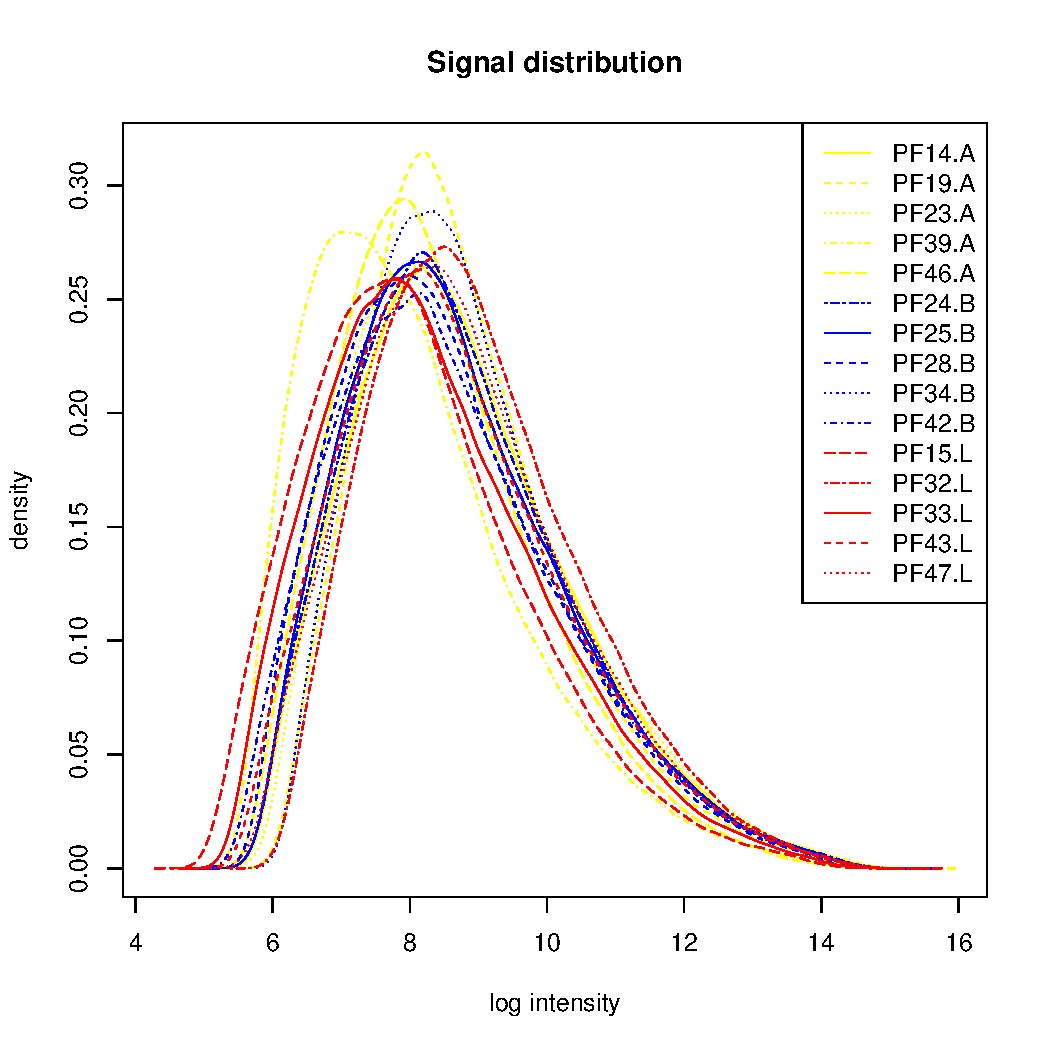
\includegraphics[width=\maxwidth]{images/graficplotHist-1} 

\end{knitrout}
\caption{Distribución de las expresiones de cada array. Aunque los gráficos muestran una cierta heterogeneidad entre muestras el aspecto de todas ellas es compatible con la "normalidad" es decir no sugieren que pueda haber algún problema en los datos.}
\end{figure}

Un diagrama de cajas muestra la misma información facilitando más la comparación entre distribuciones.
  
\begin{figure}[htbp]
\centering
\begin{knitrout}
\definecolor{shadecolor}{rgb}{0.969, 0.969, 0.969}\color{fgcolor}\begin{kframe}
\begin{alltt}
\hlkwd{boxplot}\hlstd{(rawData,} \hlkwc{cex.axis}\hlstd{=}\hlnum{0.6}\hlstd{,} \hlkwc{col}\hlstd{=colores,} \hlkwc{las}\hlstd{=}\hlnum{2}\hlstd{,} \hlkwc{names}\hlstd{=sampleNames,}
        \hlkwc{main}\hlstd{=}\hlstr{"Signal distribution for selected chips"}\hlstd{)}
\end{alltt}
\end{kframe}
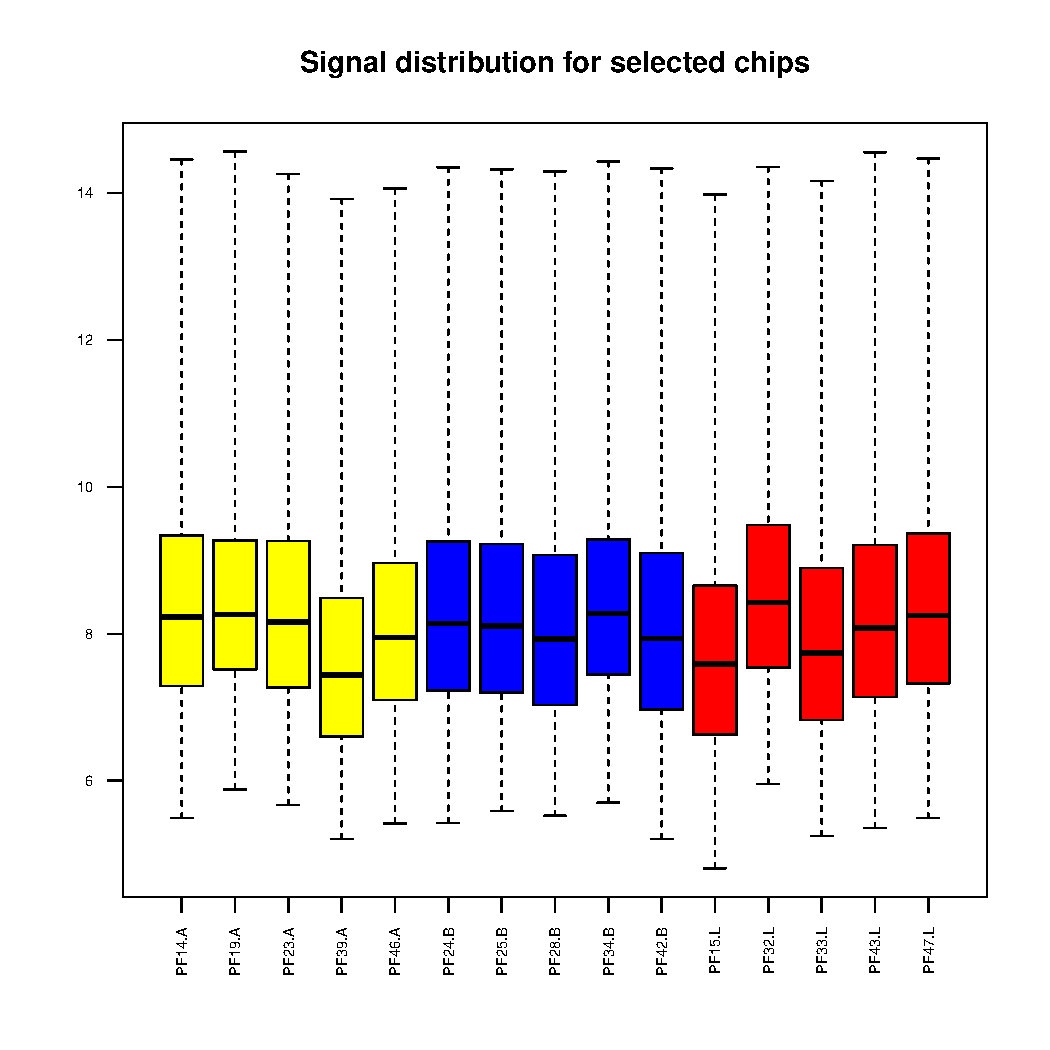
\includegraphics[width=\maxwidth]{images/graficboxplot-1} 

\end{knitrout}
  \caption{El diagrama de cajas muestra, de forma similar al histograma, cómo las distribuciones de los datos son relativamente similares. Hay heterogeneidad pero no se muestra ninguna diferencia sistemática, lo que sugiere que es conveniente normalizar peró no parece que hayan arrays problemáticos}
  \label{fig:boxplot}
\end{figure}

Una representación multivariante como la ofrecida por los gráficos de las componentes principales suele resultar muy informativa de posibles problemas como efectos batch o presencia de valores "raros". El gráfico de componentes principales muestra los datos en dimensión reducida de forma que cada componente explica una dimensión de mayor variabilidad e independiente de la siguiente. Representando el porcentaje de variabilidad explicada para cada componente tenemos una medida de la importancia de los grupos que se puedan visualizar. Si la suma de los porecentajes es alta, por ejemplo superior al 50\% las conclusiones que de ellos se deriven seran más fiables que con valores bajos, por ejemplo inferiores al 30\% de varianza explicada.

\begin{knitrout}
\definecolor{shadecolor}{rgb}{0.969, 0.969, 0.969}\color{fgcolor}\begin{kframe}
\begin{alltt}
\hlstd{plotPCA} \hlkwb{<-} \hlkwa{function} \hlstd{(} \hlkwc{X}\hlstd{,} \hlkwc{labels}\hlstd{=}\hlkwa{NULL}\hlstd{,} \hlkwc{colors}\hlstd{=}\hlkwa{NULL}\hlstd{,} \hlkwc{dataDesc}\hlstd{=}\hlstr{""}\hlstd{,} \hlkwc{scale}\hlstd{=}\hlnum{FALSE}\hlstd{)}
\hlstd{\{}
  \hlstd{pcX}\hlkwb{<-}\hlkwd{prcomp}\hlstd{(}\hlkwd{t}\hlstd{(X),} \hlkwc{scale}\hlstd{=scale)} \hlcom{# o prcomp(t(X))}
  \hlstd{loads}\hlkwb{<-} \hlkwd{round}\hlstd{(pcX}\hlopt{$}\hlstd{sdev}\hlopt{^}\hlnum{2}\hlopt{/}\hlkwd{sum}\hlstd{(pcX}\hlopt{$}\hlstd{sdev}\hlopt{^}\hlnum{2}\hlstd{)}\hlopt{*}\hlnum{100}\hlstd{,}\hlnum{1}\hlstd{)}
  \hlstd{xlab}\hlkwb{<-}\hlkwd{c}\hlstd{(}\hlkwd{paste}\hlstd{(}\hlstr{"PC1"}\hlstd{,loads[}\hlnum{1}\hlstd{],}\hlstr{"%"}\hlstd{))}
  \hlstd{ylab}\hlkwb{<-}\hlkwd{c}\hlstd{(}\hlkwd{paste}\hlstd{(}\hlstr{"PC2"}\hlstd{,loads[}\hlnum{2}\hlstd{],}\hlstr{"%"}\hlstd{))}
  \hlkwa{if} \hlstd{(}\hlkwd{is.null}\hlstd{(colors)) colors}\hlkwb{=}\hlnum{1}
  \hlkwd{plot}\hlstd{(pcX}\hlopt{$}\hlstd{x[,}\hlnum{1}\hlopt{:}\hlnum{2}\hlstd{],}\hlkwc{xlab}\hlstd{=xlab,}\hlkwc{ylab}\hlstd{=ylab,} \hlkwc{col}\hlstd{=colors,}
       \hlkwc{xlim}\hlstd{=}\hlkwd{c}\hlstd{(}\hlkwd{min}\hlstd{(pcX}\hlopt{$}\hlstd{x[,}\hlnum{1}\hlstd{])}\hlopt{-}\hlnum{10}\hlstd{,} \hlkwd{max}\hlstd{(pcX}\hlopt{$}\hlstd{x[,}\hlnum{1}\hlstd{])}\hlopt{+}\hlnum{10}\hlstd{))}
  \hlkwd{text}\hlstd{(pcX}\hlopt{$}\hlstd{x[,}\hlnum{1}\hlstd{],pcX}\hlopt{$}\hlstd{x[,}\hlnum{2}\hlstd{], labels,} \hlkwc{pos}\hlstd{=}\hlnum{3}\hlstd{,} \hlkwc{cex}\hlstd{=}\hlnum{0.8}\hlstd{)}
  \hlkwd{title}\hlstd{(}\hlkwd{paste}\hlstd{(}\hlstr{"Plot of first 2 PCs for expressions in"}\hlstd{, dataDesc,} \hlkwc{sep}\hlstd{=}\hlstr{" "}\hlstd{),} \hlkwc{cex}\hlstd{=}\hlnum{0.8}\hlstd{)}
\hlstd{\}}
\end{alltt}
\end{kframe}
\end{knitrout}

\begin{figure}[htbp]
\centering
\begin{knitrout}
\definecolor{shadecolor}{rgb}{0.969, 0.969, 0.969}\color{fgcolor}\begin{kframe}
\begin{alltt}
\hlkwd{plotPCA}\hlstd{(}\hlkwd{exprs}\hlstd{(rawData),} \hlkwc{labels}\hlstd{=sampleNames,} \hlkwc{dataDesc}\hlstd{=}\hlstr{"selected samples"}\hlstd{)}
\end{alltt}
\end{kframe}
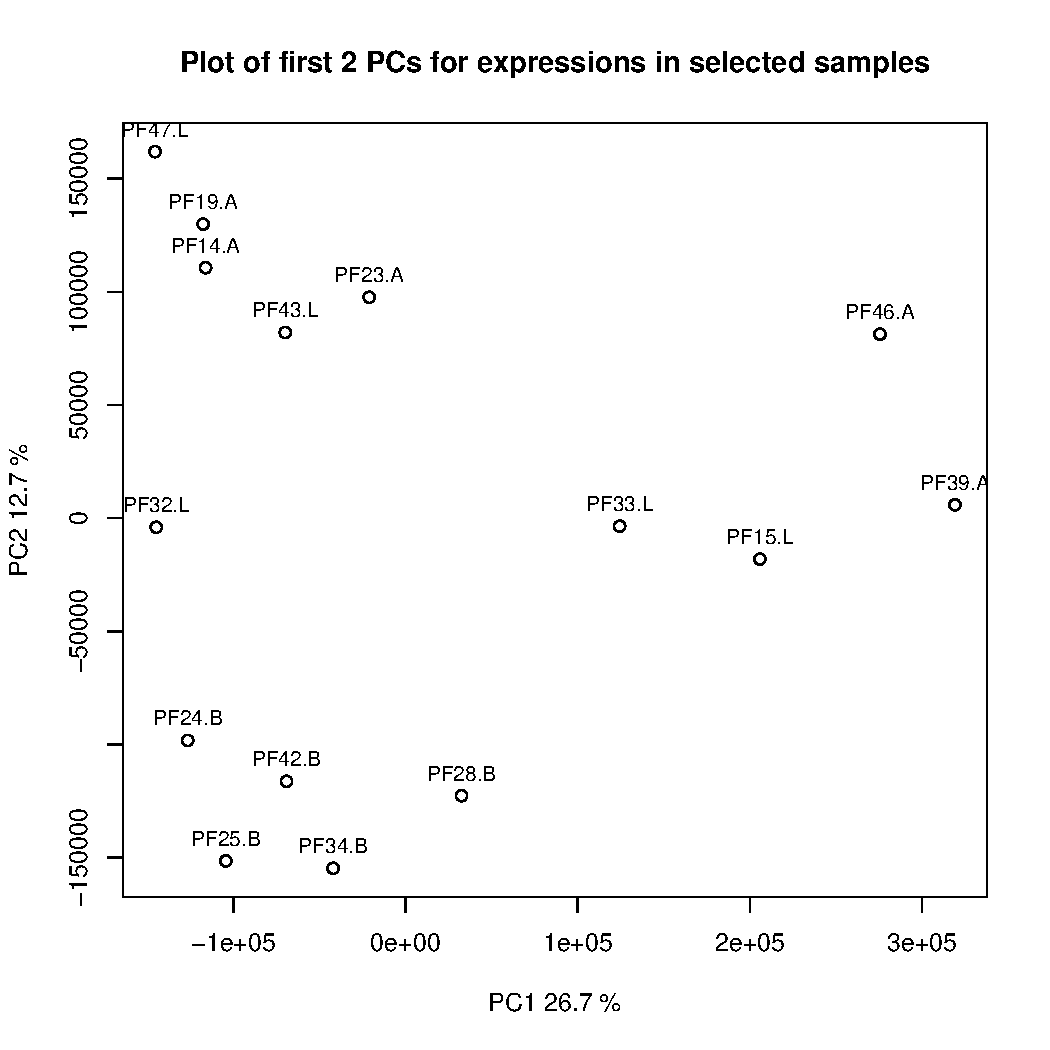
\includegraphics[width=\maxwidth]{images/graficplotPCA2D-1} 

\end{knitrout}
\caption{Representación de las dos primeras componentes de un análisi de components principales. Los grupos aparecen algo separados pero el porcentaje de variabilidad explicado por las dos primeras componentes sugiere que puede no ser muy explicativas}
\label{fig:PCA2D}
\end{figure}

Un enfoque alternativo al del PCA aunque relacionado es realizar un análisis basado en distancias. Podemos hacerlo calculando y visualizando la matriz de distancias mediante un mapa de colores o mediante un agrupamiento jerárquico seguido de un dendrograma.

\begin{figure}
\centering
\begin{knitrout}
\definecolor{shadecolor}{rgb}{0.969, 0.969, 0.969}\color{fgcolor}\begin{kframe}
\begin{alltt}
  \hlstd{manDist} \hlkwb{<-}  \hlkwd{dist}\hlstd{(}\hlkwd{t}\hlstd{(}\hlkwd{exprs}\hlstd{(rawData)))}
  \hlkwd{heatmap} \hlstd{(}\hlkwd{as.matrix}\hlstd{(manDist),}  \hlkwc{col}\hlstd{=}\hlkwd{heat.colors}\hlstd{(}\hlnum{16}\hlstd{))}
\end{alltt}
\end{kframe}
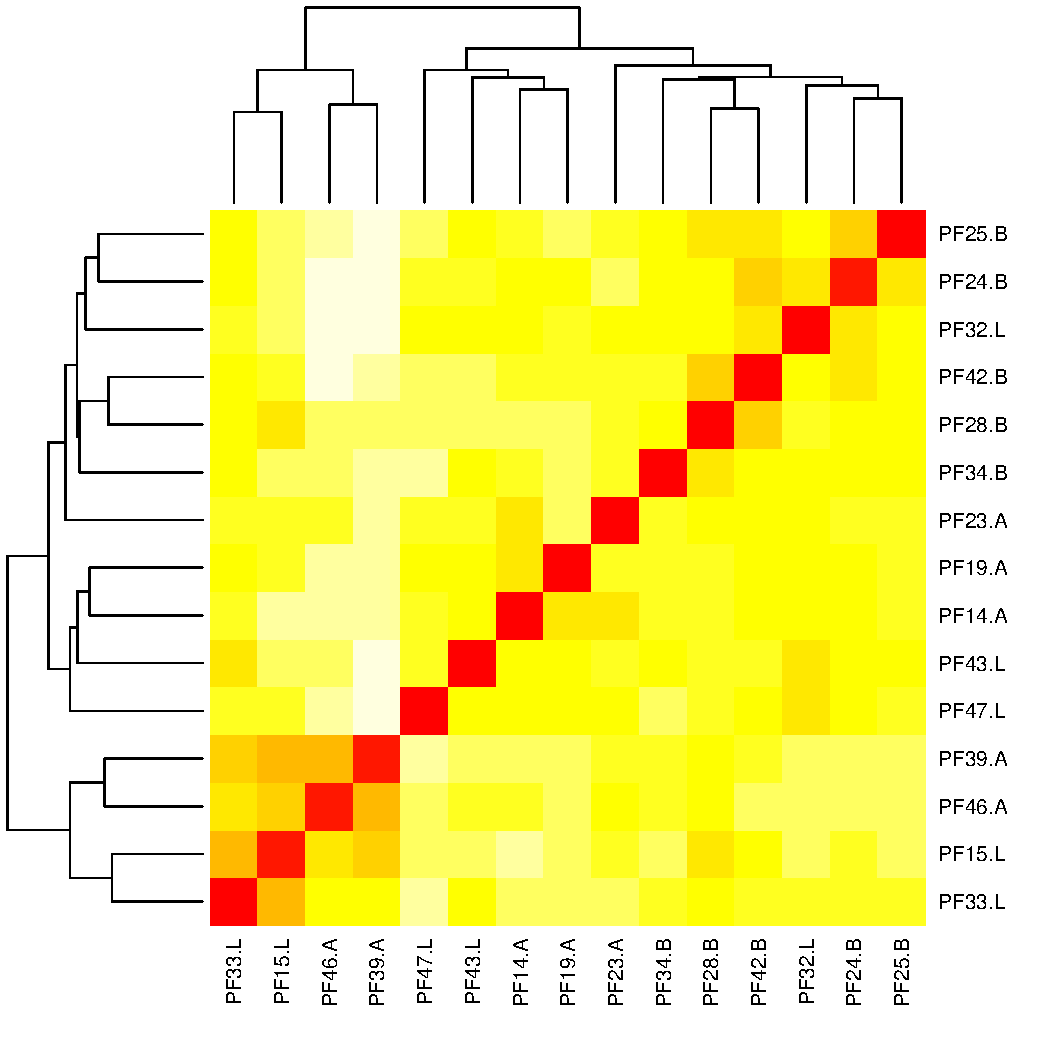
\includegraphics[width=\maxwidth]{images/graficdistAnalisis-1} 

\end{knitrout}
\caption{Mapa de colores de las distancias (euclídeas) entre los distintos arrays}
\label{fig:distArrays}
\end{figure}


Un cluster jerárquico seguido de un dendrograma nos puede ayudar a hacernos una idea de si las muestras se agrupan por condiciones experimentales. 

Si lo hacen es bueno, pero si no, no es necesariamente indicador de problemas, 
puesto que es un gráfico basado en todo los datos.

\begin{figure}
\centering
\begin{knitrout}
\definecolor{shadecolor}{rgb}{0.969, 0.969, 0.969}\color{fgcolor}
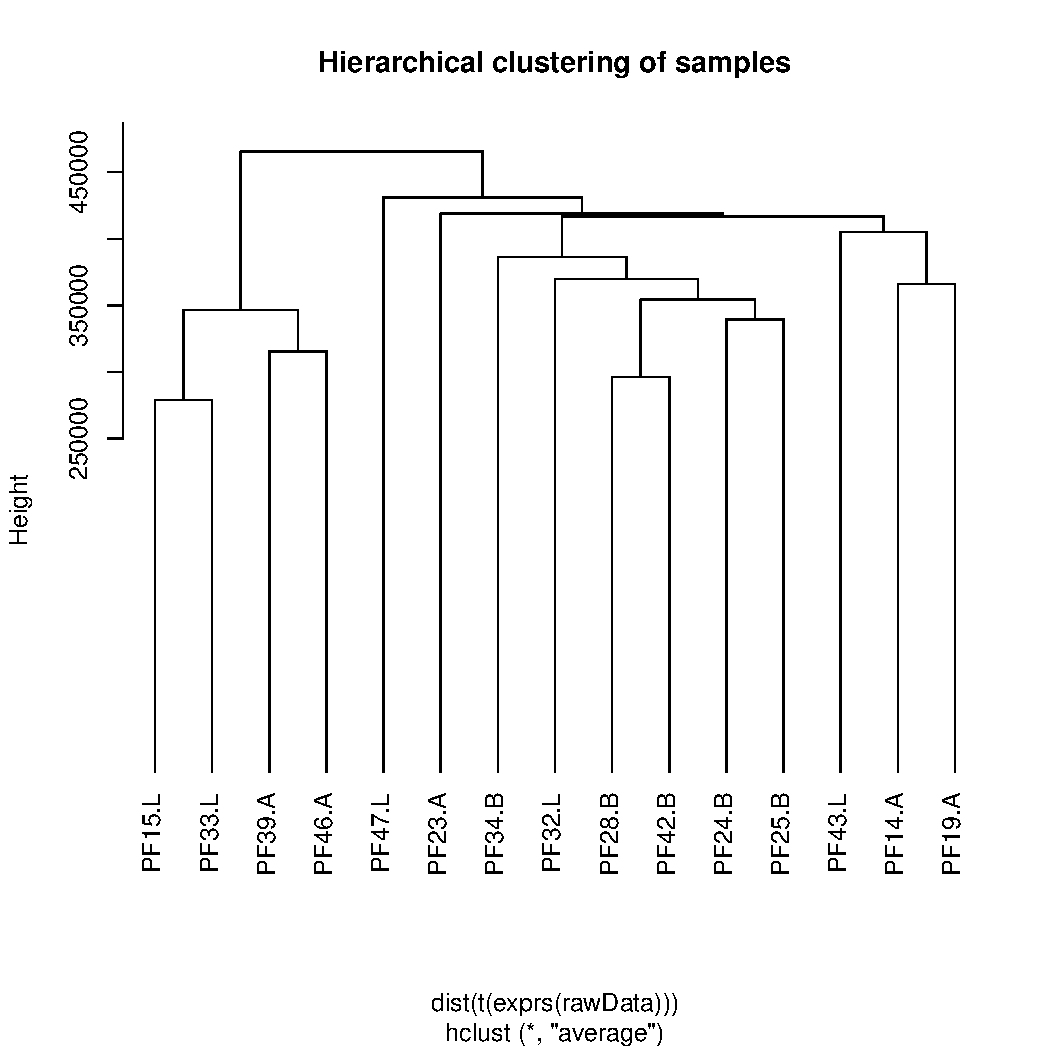
\includegraphics[width=\maxwidth]{images/graficplotDendro-1} 

\end{knitrout}
\caption{Dendrograma resultante de un agrupamiento jerárquico entre las muestras.
  Como en otras representaciones (Heatmaps, PCA) se observa una cierta agrupación de muestras de tipos similares aunque también una cierta heterogeneidad, atribuïble probablemente a la diferencia entre pacientes}
\label{fig:dendrograma}
\end{figure}

\subsubsection{Control de calidad (2): métodos específicos para microarrays}


Las exploraciones anteriores nos proporcionan una idea general acerca de la distribución de los datos y la posible presencia de grupos naturales (e.g. por tratamientos) o artificiales (ej. días de procesad).

Existen también métodos para el control de calidad específicos de microarrays, como por ejemplo:
\begin{itemize}
\item Los controles de calidad estándar de Affymetrix, descritos en el paquete \Rpackage{simpleaffy}.
\item Controles basados en modelos a nivel de sondas,  descritos en el paquete \Rpackage{affyPLM}.
\end{itemize}

De entre los controles de calidad ``estándar'' de affymetrix nos fijaremos en el gráfico de degradación que permite hacerse una idea de como ha sido el 
proceso de hibridación de las muestras. Si las líneas que forman el gráfico son más o menos paralelas sugiere una calidad similar en todos los arrays.



\begin{figure}[htbp]
 \centering
\begin{knitrout}
\definecolor{shadecolor}{rgb}{0.969, 0.969, 0.969}\color{fgcolor}
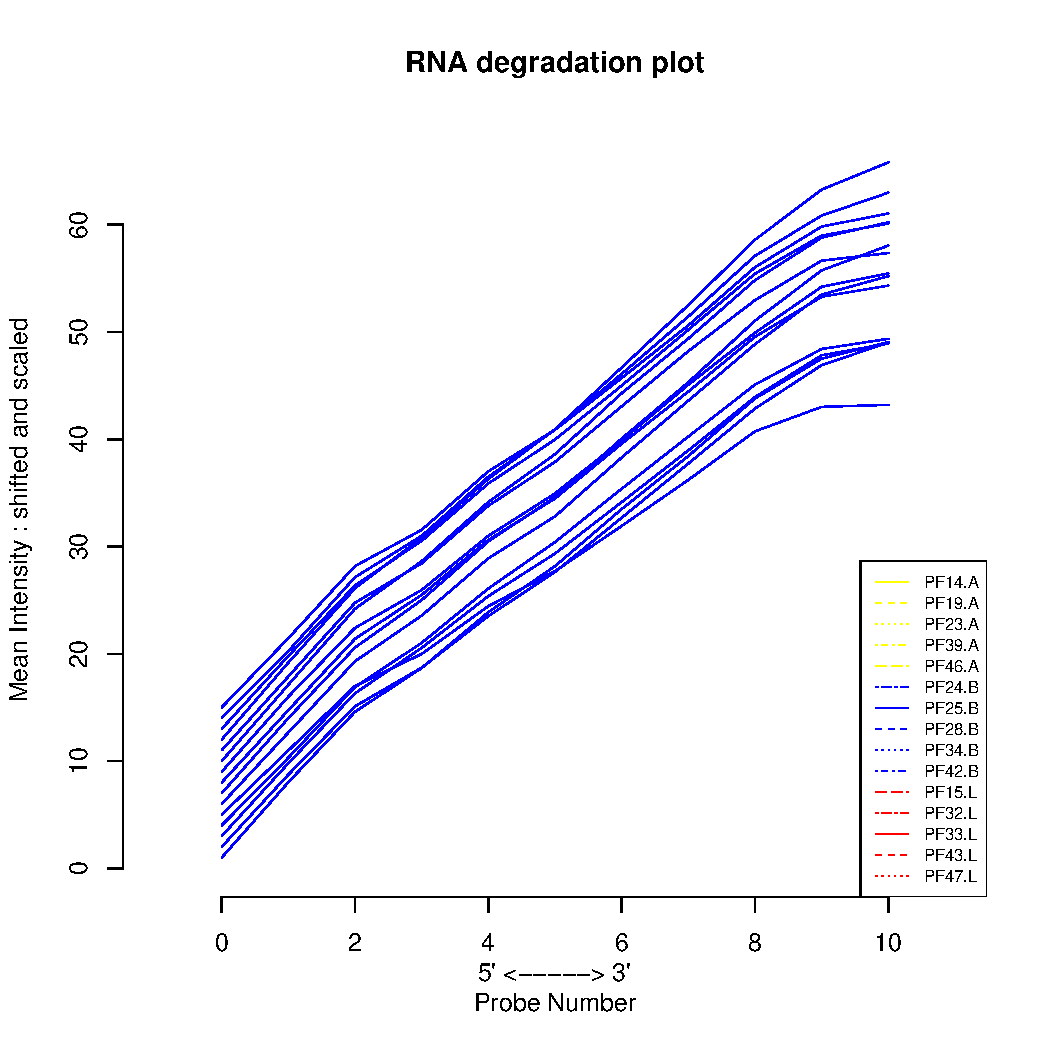
\includegraphics[width=\maxwidth]{images/graficplotDeg-1} 

\end{knitrout}
\caption{Gráfico de degradación. Las lineas paralelas muestran que el nivel de degradación del RNA es similar en todos los chips.}
\label{fig:degeadationPlot}
\end{figure}

El ``probe-level-model analysis'' ajusta un model a la intensidad de las sondas y analiza los residuos de este ajuste a traves de dos graficos: el RLE -de expresiones relativas-- y el NUSE --de residuos centrados y normalizados-- (vease \cite{Gentleman:2005}). 
Si los datos son de calidad ambos graficos deben ser centrados y relativamente simetricos. Cambios en esta situacion sugieren problemas en los arrays que no las verifiquen. Estos métodos se encuentran implementados en el paquete \Rpackage{affyPLM}.


\begin{knitrout}
\definecolor{shadecolor}{rgb}{0.969, 0.969, 0.969}\color{fgcolor}\begin{kframe}
\begin{alltt}
\hlkwd{stopifnot}\hlstd{(}\hlkwd{require}\hlstd{(affyPLM))}
\hlkwa{if} \hlstd{(}\hlopt{!}\hlstd{(}\hlkwd{exists}\hlstd{(}\hlstr{"Pset"}\hlstd{)))}
  \hlstd{Pset}\hlkwb{<-} \hlkwd{fitPLM}\hlstd{(rawData)}
\end{alltt}
\end{kframe}
\end{knitrout}


\begin{figure}[htbp]
 \centering
\begin{knitrout}
\definecolor{shadecolor}{rgb}{0.969, 0.969, 0.969}\color{fgcolor}
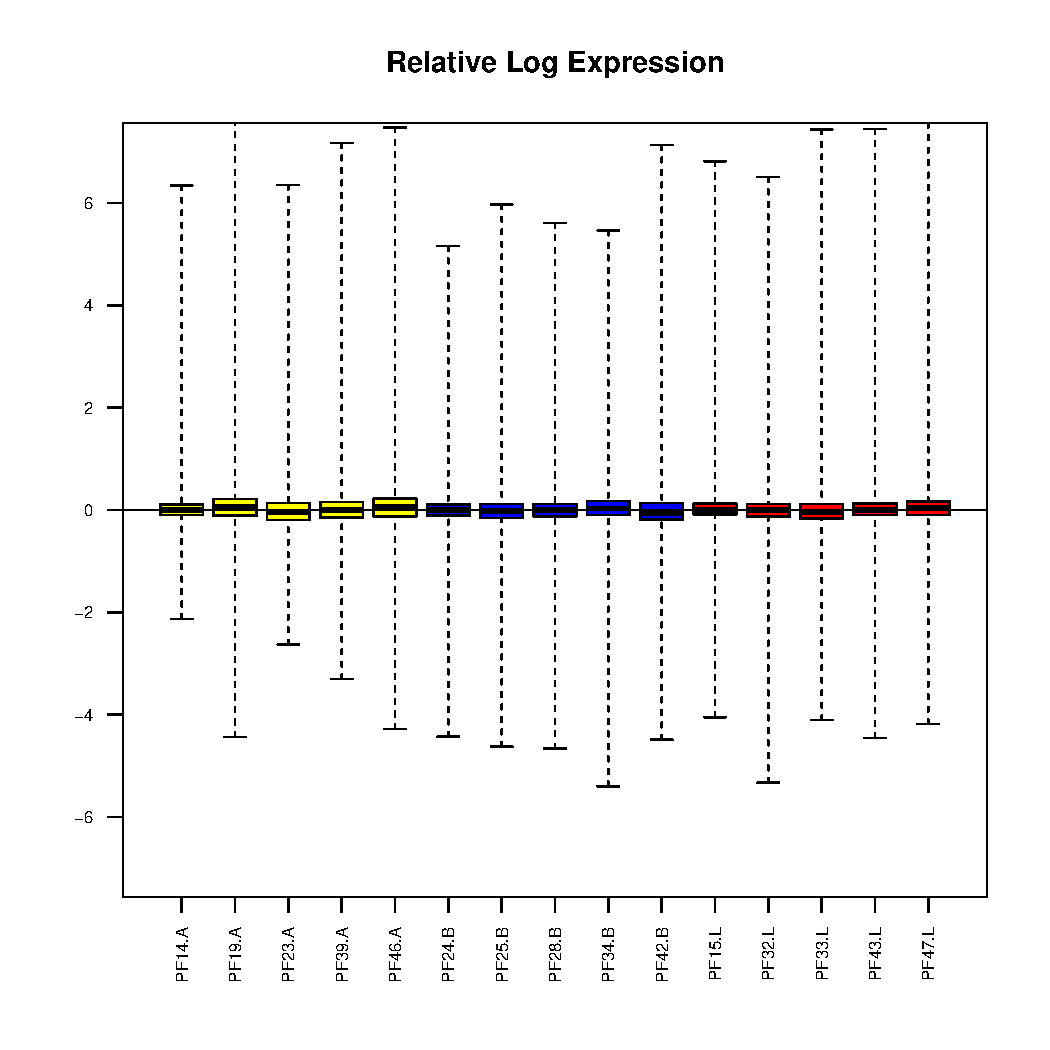
\includegraphics[width=\maxwidth]{images/graficplotRLE-1} 

\end{knitrout}
\caption{Gráfico de expresiones relativas (RLE) resultante del análisis basado en modelos (PLM). Las muestras son simétricas y similares lo que sugiera una calidad aceptable de los datos}
\label{fig:RLE}
\end{figure}


\begin{figure}[htbp]
 \centering
\begin{knitrout}
\definecolor{shadecolor}{rgb}{0.969, 0.969, 0.969}\color{fgcolor}
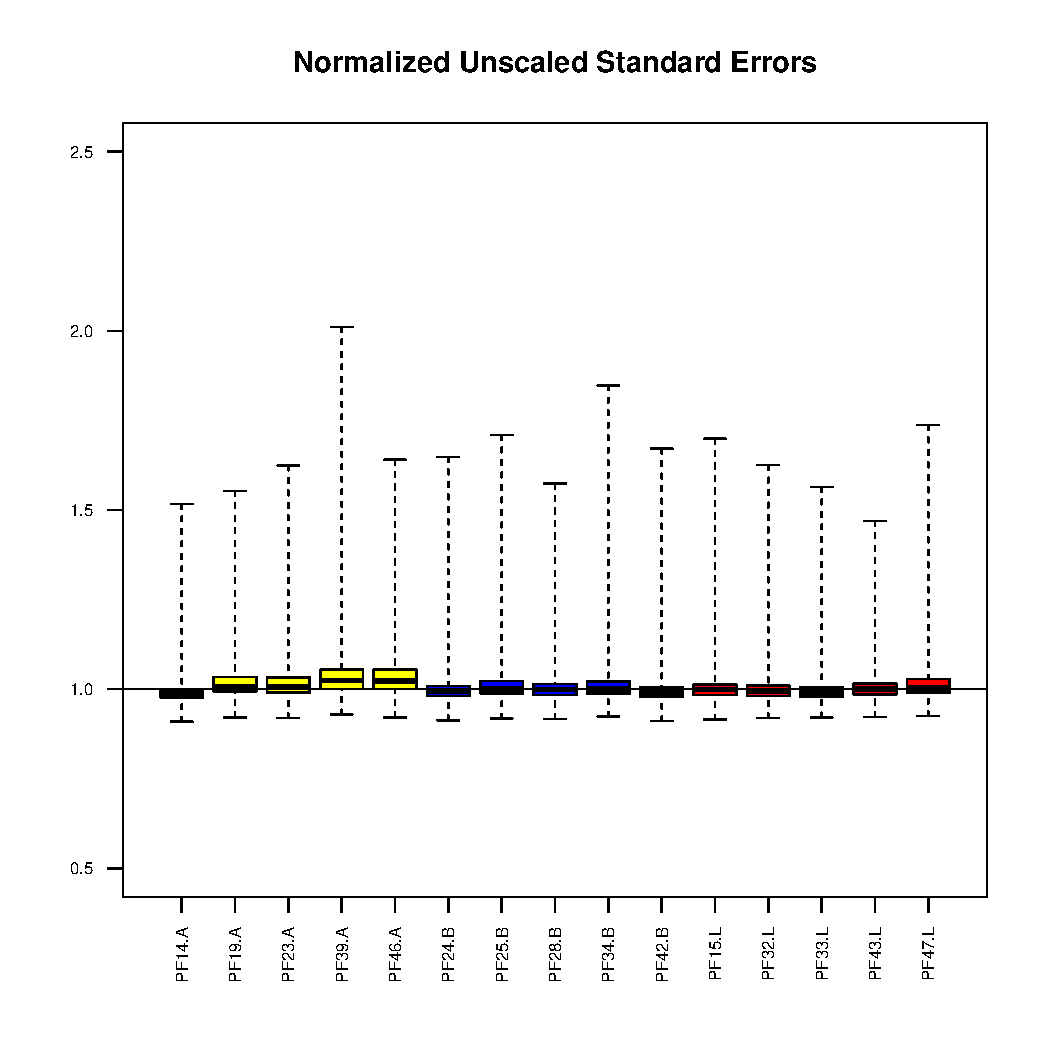
\includegraphics[width=\maxwidth]{images/graficplotNUSE-1} 

\end{knitrout}
\caption{Gráfico de errores estandarizados normalizados provenientes de los residuos del análisis basado en modelos (PLM).
 No aparece ninguna caja \emph{claramente} diferenciada de las otras lo que sugiera una calidad aceptable de los datos}
\label{fig:RLE}
\end{figure}

\subsubsection{Paquetes ``all-in-one'' para el control de calidad''}

El paquete \Rpackage{arrayQualitMetrics} encapsula todos los análisis anteriores, y alguno más, facilitando su ejecución e incluso su interpretación. La instrucción \texttt{arrayQualityMetrics} lleva a cabo todos los análisi de golpe y genera un informe de resultados con ayudas a la interpretación y a la detección de arrays problemáticos.

\begin{knitrout}
\definecolor{shadecolor}{rgb}{0.969, 0.969, 0.969}\color{fgcolor}\begin{kframe}
\begin{alltt}
\hlkwd{stopifnot}\hlstd{(}\hlkwd{require}\hlstd{(arrayQualityMetrics))}
\hlkwd{arrayQualityMetrics}\hlstd{(rawData,} \hlkwc{outdir} \hlstd{=} \hlkwd{file.path}\hlstd{(resultsDir,} \hlstr{"Qual/arrayQuality"}\hlstd{),}
                    \hlkwc{force}\hlstd{=}\hlnum{TRUE}\hlstd{)}
\end{alltt}


{\ttfamily\noindent\itshape\color{messagecolor}{\#\# The directory '/home/alex/Dropbox (VHIR)/Scripts/Exemple\_Analisis\_BioC/results/Qual/arrayQuality' has been created.}}

{\ttfamily\noindent\color{warningcolor}{\#\# Warning in svgStyleAttributes(style): Removing non-SVG style attribute name(s): subscripts, group.number, group.value}}

{\ttfamily\noindent\color{warningcolor}{\#\# Warning in svgStyleAttributes(style): Removing non-SVG style attribute name(s): subscripts, group.number, group.value}}

{\ttfamily\noindent\color{warningcolor}{\#\# Warning in svgStyleAttributes(style): Removing non-SVG style attribute name(s): subscripts, group.number, group.value}}

{\ttfamily\noindent\color{warningcolor}{\#\# Warning in svgStyleAttributes(style): Removing non-SVG style attribute name(s): subscripts, group.number, group.value}}

{\ttfamily\noindent\color{warningcolor}{\#\# Warning in svgStyleAttributes(style): Removing non-SVG style attribute name(s): subscripts, group.number, group.value}}

{\ttfamily\noindent\color{warningcolor}{\#\# Warning in svgStyleAttributes(style): Removing non-SVG style attribute name(s): subscripts, group.number, group.value}}

{\ttfamily\noindent\color{warningcolor}{\#\# Warning in svgStyleAttributes(style): Removing non-SVG style attribute name(s): subscripts, group.number, group.value}}

{\ttfamily\noindent\color{warningcolor}{\#\# Warning in svgStyleAttributes(style): Removing non-SVG style attribute name(s): subscripts, group.number, group.value}}

{\ttfamily\noindent\color{warningcolor}{\#\# Warning in svgStyleAttributes(style): Removing non-SVG style attribute name(s): subscripts, group.number, group.value}}

{\ttfamily\noindent\color{warningcolor}{\#\# Warning in svgStyleAttributes(style): Removing non-SVG style attribute name(s): subscripts, group.number, group.value}}

{\ttfamily\noindent\color{warningcolor}{\#\# Warning in svgStyleAttributes(style): Removing non-SVG style attribute name(s): subscripts, group.number, group.value}}

{\ttfamily\noindent\color{warningcolor}{\#\# Warning in svgStyleAttributes(style): Removing non-SVG style attribute name(s): subscripts, group.number, group.value}}

{\ttfamily\noindent\color{warningcolor}{\#\# Warning in svgStyleAttributes(style): Removing non-SVG style attribute name(s): subscripts, group.number, group.value}}

{\ttfamily\noindent\color{warningcolor}{\#\# Warning in svgStyleAttributes(style): Removing non-SVG style attribute name(s): subscripts, group.number, group.value}}

{\ttfamily\noindent\color{warningcolor}{\#\# Warning in svgStyleAttributes(style): Removing non-SVG style attribute name(s): subscripts, group.number, group.value}}

{\ttfamily\noindent\color{warningcolor}{\#\# Warning in KernSmooth::bkde2D(x, gridsize = nbin, bandwidth = bandwidth): Binning grid too coarse for current (small) bandwidth: consider increasing 'gridsize'}}

{\ttfamily\noindent\color{warningcolor}{\#\# Warning in KernSmooth::bkde2D(x, gridsize = nbin, bandwidth = bandwidth): Binning grid too coarse for current (small) bandwidth: consider increasing 'gridsize'}}

{\ttfamily\noindent\color{warningcolor}{\#\# Warning in KernSmooth::bkde2D(x, gridsize = nbin, bandwidth = bandwidth): Binning grid too coarse for current (small) bandwidth: consider increasing 'gridsize'}}

{\ttfamily\noindent\color{warningcolor}{\#\# Warning in KernSmooth::bkde2D(x, gridsize = nbin, bandwidth = bandwidth): Binning grid too coarse for current (small) bandwidth: consider increasing 'gridsize'}}

{\ttfamily\noindent\color{warningcolor}{\#\# Warning in KernSmooth::bkde2D(x, gridsize = nbin, bandwidth = bandwidth): Binning grid too coarse for current (small) bandwidth: consider increasing 'gridsize'}}

{\ttfamily\noindent\color{warningcolor}{\#\# Warning in KernSmooth::bkde2D(x, gridsize = nbin, bandwidth = bandwidth): Binning grid too coarse for current (small) bandwidth: consider increasing 'gridsize'}}

{\ttfamily\noindent\color{warningcolor}{\#\# Warning in KernSmooth::bkde2D(x, gridsize = nbin, bandwidth = bandwidth): Binning grid too coarse for current (small) bandwidth: consider increasing 'gridsize'}}

{\ttfamily\noindent\color{warningcolor}{\#\# Warning in KernSmooth::bkde2D(x, gridsize = nbin, bandwidth = bandwidth): Binning grid too coarse for current (small) bandwidth: consider increasing 'gridsize'}}

{\ttfamily\noindent\color{warningcolor}{\#\# Warning in KernSmooth::bkde2D(x, gridsize = nbin, bandwidth = bandwidth): Binning grid too coarse for current (small) bandwidth: consider increasing 'gridsize'}}

{\ttfamily\noindent\color{warningcolor}{\#\# Warning in KernSmooth::bkde2D(x, gridsize = nbin, bandwidth = bandwidth): Binning grid too coarse for current (small) bandwidth: consider increasing 'gridsize'}}

{\ttfamily\noindent\color{warningcolor}{\#\# Warning in KernSmooth::bkde2D(x, gridsize = nbin, bandwidth = bandwidth): Binning grid too coarse for current (small) bandwidth: consider increasing 'gridsize'}}

{\ttfamily\noindent\color{warningcolor}{\#\# Warning in KernSmooth::bkde2D(x, gridsize = nbin, bandwidth = bandwidth): Binning grid too coarse for current (small) bandwidth: consider increasing 'gridsize'}}

{\ttfamily\noindent\color{warningcolor}{\#\# Warning in KernSmooth::bkde2D(x, gridsize = nbin, bandwidth = bandwidth): Binning grid too coarse for current (small) bandwidth: consider increasing 'gridsize'}}

{\ttfamily\noindent\color{warningcolor}{\#\# Warning in KernSmooth::bkde2D(x, gridsize = nbin, bandwidth = bandwidth): Binning grid too coarse for current (small) bandwidth: consider increasing 'gridsize'}}

{\ttfamily\noindent\color{warningcolor}{\#\# Warning in KernSmooth::bkde2D(x, gridsize = nbin, bandwidth = bandwidth): Binning grid too coarse for current (small) bandwidth: consider increasing 'gridsize'}}

{\ttfamily\noindent\color{warningcolor}{\#\# Warning in KernSmooth::bkde2D(x, gridsize = nbin, bandwidth = bandwidth): Binning grid too coarse for current (small) bandwidth: consider increasing 'gridsize'}}\end{kframe}
\end{knitrout}

\subsubsection{Archivos con los resultados del control de calidad}

Los resultados del control de calidad realizado con \texttt{arrayQualityMetrics} se encuentran  accesibles a traves del archivo \texttt{index.html} contenido en el subdirectorio creado al invocarlo -en este caso denominado \texttt{arrayQuality}.


\subsection{Normalizacion y Filtraje}

Una vez realizado el control de calidad se procede a normalizar los datos y sumarizarlos.

La normalización puede hacerse por distintos métodos (MAS5, VSN, RMA, GCRMA, ...) pero en este caso se utilizará el método RMA que es sin duda el más utilizado entre arrays de affymetrix.

El procesado mediante RMA implica un proceso en tres etapas: 
\begin{itemize}
\item Corrección de fondo (el RMA hace precisamente esto).
\item Normalización para hacer los valores de los arrays comparables.
\item Summarización de las diversas sondas asociadas a cada grupo de sondas para dar un único valor.
\end{itemize}


\begin{knitrout}
\definecolor{shadecolor}{rgb}{0.969, 0.969, 0.969}\color{fgcolor}\begin{kframe}
\begin{alltt}
\hlkwd{stopifnot}\hlstd{(}\hlkwd{require}\hlstd{(affy))}
\hlstd{eset_rma} \hlkwb{<-} \hlkwd{rma}\hlstd{(rawData)}
\end{alltt}
\begin{verbatim}
## Background correcting
## Normalizing
## Calculating Expression
\end{verbatim}
\end{kframe}
\end{knitrout}

Un boxplot de los valores normalizados muestra que los valores han quedado claramente en una escala común en donde se pueden comparar.
\begin{figure}[htbp]
\centering
\begin{knitrout}
\definecolor{shadecolor}{rgb}{0.969, 0.969, 0.969}\color{fgcolor}\begin{kframe}
\begin{alltt}
\hlkwd{boxplot}\hlstd{(eset_rma,}\hlkwc{main}\hlstd{=}\hlstr{"RMA"}\hlstd{,} \hlkwc{names}\hlstd{=sampleNames,} \hlkwc{cex.axis}\hlstd{=}\hlnum{0.7}\hlstd{,} \hlkwc{col}\hlstd{=colores,}\hlkwc{las}\hlstd{=}\hlnum{2}\hlstd{)}
\end{alltt}
\end{kframe}
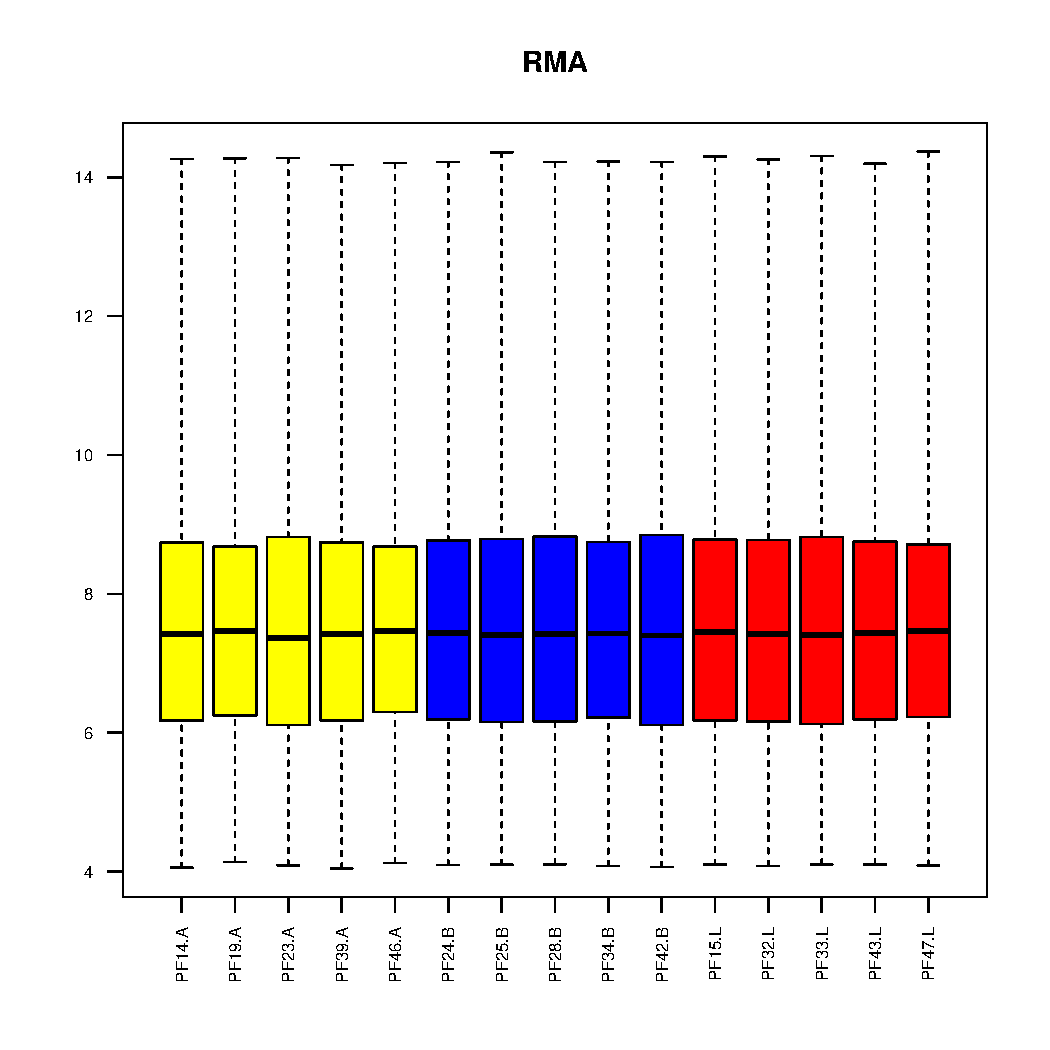
\includegraphics[width=\maxwidth]{images/graficnormBoxPlot-1} 

\end{knitrout}
\caption{El diagrama de cajas después de normalizar muestra como dicho proceso ha puesto los valores en una escala completamente comparable. \emph{Esto no significa que si hubieran errores los habría arreglado} por lo que dicho proceso debe hacerse tras descartar la ausencia de arrays problemáticos}
\label{fig:boxplot}
\end{figure}

\subsubsection{Filtraje}

El filtraje \emph{no específico} permite eliminar los genes que varían poco entre condiciones o que deseamos quitar por otras razones como por ejemplo que no disponemos de anotación para ellos. La función \texttt{nsFilter} permite eliminar los genes que, o bien varían poco, o bien no se dispone de anotación para ellos.

Si al filtrar deseamos usar las anotaciones, o la falta de ellas, como criterio de filtraje debemos disponer del correspondiente paquete de anotaciones.

\begin{knitrout}
\definecolor{shadecolor}{rgb}{0.969, 0.969, 0.969}\color{fgcolor}\begin{kframe}
\begin{alltt}
\hlkwd{require}\hlstd{(genefilter)}
\hlstd{filtered} \hlkwb{<-} \hlkwd{nsFilter}\hlstd{(eset_rma,} \hlkwc{require.entrez}\hlstd{=}\hlnum{TRUE}\hlstd{,}
         \hlkwc{remove.dupEntrez}\hlstd{=}\hlnum{TRUE}\hlstd{,} \hlkwc{var.func}\hlstd{=IQR,}
         \hlkwc{var.cutoff}\hlstd{=}\hlnum{0.5}\hlstd{,} \hlkwc{var.filter}\hlstd{=}\hlnum{TRUE}\hlstd{,}
         \hlkwc{filterByQuantile}\hlstd{=}\hlnum{TRUE}\hlstd{,} \hlkwc{feature.exclude}\hlstd{=}\hlstr{"^AFFX"}\hlstd{)}
\end{alltt}
\end{kframe}
\end{knitrout}

La función \texttt{nsFilter} devuelve los valores filtrados en un objeto \texttt{expressionSet} y un informe de los resultados del filtraje.

\begin{knitrout}
\definecolor{shadecolor}{rgb}{0.969, 0.969, 0.969}\color{fgcolor}\begin{kframe}
\begin{alltt}
\hlkwd{names}\hlstd{(filtered)}
\end{alltt}
\begin{verbatim}
## [1] "eset"       "filter.log"
\end{verbatim}
\begin{alltt}
\hlkwd{class}\hlstd{(filtered}\hlopt{$}\hlstd{eset)}
\end{alltt}
\begin{verbatim}
## [1] "ExpressionSet"
## attr(,"package")
## [1] "Biobase"
\end{verbatim}
\begin{alltt}
\hlkwd{print}\hlstd{(filtered}\hlopt{$}\hlstd{filter.log)}
\end{alltt}
\begin{verbatim}
## $numDupsRemoved
## [1] 7402
## 
## $numLowVar
## [1] 6217
## 
## $numRemoved.ENTREZID
## [1] 2437
## 
## $feature.exclude
## [1] 10
\end{verbatim}
\begin{alltt}
\hlstd{eset_filtered} \hlkwb{<-}\hlstd{filtered}\hlopt{$}\hlstd{eset}
\end{alltt}
\end{kframe}
\end{knitrout}

Podemos grabar el objeto \texttt{eset_rma} y los datos filtrados para su posterior uso.


\subsubsection{Archivos de resultados normalizados}

El resultado de la normalización y el filtraje es un objeto \texttt{expressionSet} almacenado en un archivo binario \texttt{datos.normaliados.Rda}, que será la base para todos los estudios posteriores.

\begin{knitrout}
\definecolor{shadecolor}{rgb}{0.969, 0.969, 0.969}\color{fgcolor}\begin{kframe}
\begin{alltt}
\hlkwd{save}\hlstd{(eset_rma, eset_filtered,} \hlkwc{file}\hlstd{=}\hlkwd{file.path}\hlstd{(resultsDir,} \hlstr{"datos.normalizados.Rda"}\hlstd{))}
\end{alltt}
\end{kframe}
\end{knitrout}


Es muy común también que los investigadores deseen ver los datos normalizados por lo que también se pueden guardar en un archivo de texto para facilitar su posterior inspección. El archivo \texttt{Datos.Normalizados.Filtrados.csv2} contiene los datos normalizados y filtrados separados por ``;'' para no generar problemas de formato con el punto decimal en ingles o español.

\begin{knitrout}
\definecolor{shadecolor}{rgb}{0.969, 0.969, 0.969}\color{fgcolor}\begin{kframe}
\begin{alltt}
\hlkwd{write.csv2}\hlstd{(}\hlkwd{exprs}\hlstd{(eset_rma),} \hlkwd{file.path}\hlstd{(resultsDir,} \hlstr{"Datos.Normalizados.csv2"}\hlstd{))}
\end{alltt}
\end{kframe}
\end{knitrout}


\section{Selección de genes diferencialmente expresados}

Como en las etapas anteriores la selección de genes diferencialmente expresados (GDE)
puede basarse en distintas aproximaciones, desde la $t$ de Student al programa SAM pasando por multitud de variantes.

En este ejemplo, dado que se realizaran tres comparaciones que luego deseamos comparar entre ellas, se aplicará la aproximación presentada por Smyth \emph{et al.} (2004) basado 
en la utilización del \emph{modelo lineal general} combinada con un método 
para obtener una estimación mejorada de la varianza. 

\subsection{Análisis basado en modelos lineales}


\subsubsection{Matrices de diseño y de contrastes}

El primer paso para el análisis basado en modelos lineales es crear la matriz de diseño.
Básicamente se trata de una tabla que describe la asignación de cada muestra a un grupo. Tiene tantas filas como muestras y tantas columnas como grupos (si solo se considera un factor)Cada fila contiene un uno en la columna del grupo al que pertenece la muestra y un cero en las restantes.

La matriz de contrastes esse utiliza para describir las comparaciones entre grupos. Consta de tantas columnas como comparaciones y tantas filas como grupos (es decir como columnas de la matriz de diseño). Una comparación entre grupos --lamada ``contraste''-- se representa con un ``1'' y un ``-1'' en las filas de los grupos a comparar y ceros en las restantes. Si varios grupos intervinieran en la comparación se tendría tantos coeeficientes como grupos con la única restricción de que su suma sería cero. 

La matriz de diseño puede definirse manualmente o a partir de un factor 
creado específicamente para ello.

Manualmente, seria:
\begin{knitrout}
\definecolor{shadecolor}{rgb}{0.969, 0.969, 0.969}\color{fgcolor}\begin{kframe}
\begin{alltt}
\hlstd{design}\hlkwb{<-}\hlkwd{matrix}\hlstd{(}
            \hlkwd{c}\hlstd{(}\hlnum{1}\hlstd{,}\hlnum{1}\hlstd{,}\hlnum{1}\hlstd{,}\hlnum{1}\hlstd{,}\hlnum{1}\hlstd{,}\hlnum{0}\hlstd{,}\hlnum{0}\hlstd{,}\hlnum{0}\hlstd{,}\hlnum{0}\hlstd{,}\hlnum{0}\hlstd{,}\hlnum{0}\hlstd{,}\hlnum{0}\hlstd{,}\hlnum{0}\hlstd{,}\hlnum{0}\hlstd{,}\hlnum{0}\hlstd{,}
              \hlnum{0}\hlstd{,}\hlnum{0}\hlstd{,}\hlnum{0}\hlstd{,}\hlnum{0}\hlstd{,}\hlnum{0}\hlstd{,}\hlnum{1}\hlstd{,}\hlnum{1}\hlstd{,}\hlnum{1}\hlstd{,}\hlnum{1}\hlstd{,}\hlnum{1}\hlstd{,}\hlnum{0}\hlstd{,}\hlnum{0}\hlstd{,}\hlnum{0}\hlstd{,}\hlnum{0}\hlstd{,}\hlnum{0}\hlstd{,}
              \hlnum{0}\hlstd{,}\hlnum{0}\hlstd{,}\hlnum{0}\hlstd{,}\hlnum{0}\hlstd{,}\hlnum{0}\hlstd{,}\hlnum{0}\hlstd{,}\hlnum{0}\hlstd{,}\hlnum{0}\hlstd{,}\hlnum{0}\hlstd{,}\hlnum{0}\hlstd{,}\hlnum{1}\hlstd{,}\hlnum{1}\hlstd{,}\hlnum{1}\hlstd{,}\hlnum{1}\hlstd{,}\hlnum{1}\hlstd{),}
            \hlkwc{nrow}\hlstd{=}\hlnum{15}\hlstd{,}\hlkwc{byrow}\hlstd{=F)}
\hlkwd{colnames}\hlstd{(design)}\hlkwb{<-}\hlkwd{c}\hlstd{(}\hlstr{"A"}\hlstd{,} \hlstr{"B"}\hlstd{,} \hlstr{"L"}\hlstd{)}
\hlkwd{rownames}\hlstd{(design)} \hlkwb{<-}  \hlstd{sampleNames}
\hlkwd{print}\hlstd{(design)}
\end{alltt}
\begin{verbatim}
##        A B L
## PF14.A 1 0 0
## PF19.A 1 0 0
## PF23.A 1 0 0
## PF39.A 1 0 0
## PF46.A 1 0 0
## PF24.B 0 1 0
## PF25.B 0 1 0
## PF28.B 0 1 0
## PF34.B 0 1 0
## PF42.B 0 1 0
## PF15.L 0 0 1
## PF32.L 0 0 1
## PF33.L 0 0 1
## PF43.L 0 0 1
## PF47.L 0 0 1
\end{verbatim}
\end{kframe}
\end{knitrout}

Las comparaciones que nos interesan son las diferencias, dos a dos entre cada tipo de tumor lo que puede hacerse con los contrastes siguientes:

\begin{knitrout}
\definecolor{shadecolor}{rgb}{0.969, 0.969, 0.969}\color{fgcolor}\begin{kframe}
\begin{alltt}
\hlkwd{require}\hlstd{(limma)}
\hlstd{cont.matrix} \hlkwb{<-} \hlkwd{makeContrasts} \hlstd{(}
      \hlkwc{AvsB} \hlstd{= B}\hlopt{-}\hlstd{A,}
      \hlkwc{AvsL} \hlstd{= L}\hlopt{-}\hlstd{A,}
      \hlkwc{BvsL} \hlstd{= L}\hlopt{-}\hlstd{B,}
      \hlkwc{levels}\hlstd{=design)}
\hlkwd{print}\hlstd{(cont.matrix)}
\end{alltt}
\begin{verbatim}
##       Contrasts
## Levels AvsB AvsL BvsL
##      A   -1   -1    0
##      B    1    0   -1
##      L    0    1    1
\end{verbatim}
\end{kframe}
\end{knitrout}

\subsubsection{Estimación del modelo y selección de genes}

Una vez definida la matriz de diseño y los contrastes podemos pasar a estimar 
el modelo, estimar los contrastes y realizar las pruebas de significación 
que nos indiquen, para cada gen y cada comparación, 
si puede considerarse diferencialmente expresado.



El método implementado en \Rpackage {limma} amplía el análisis tradicional 
utilizando modelos de Bayes empíricos para combinar la información de toda la matriz de datos y de cada gen individual y  obtener estimaciones de error mejoradas.

El análisis proporciona los estadísticos de test habituales como \texttt{Fold--change}
$t$-moderados o $p$-valores ajustados que se utilizan para ordenar los genes de mas a menos diferencialmente expresados.

A fin de controlar el porcentaje de falsos positivos que puedan resultar del alto numero de contrastes realizados simultaneamente
los p--valores se ajustan de forma que tengamos control sobre la tasa de falsos positivos utilizando el metodo 
de Benjamini y Hochberg (\cite{BenjaminiHochberg:1995}). 

La funcion \texttt{topTable} genera para cada contraste una lista de genes 
ordenados de mas a menos diferencialmente expresados.

\begin{knitrout}
\definecolor{shadecolor}{rgb}{0.969, 0.969, 0.969}\color{fgcolor}\begin{kframe}
\begin{alltt}
\hlstd{topTab_AvsB} \hlkwb{<-} \hlkwd{topTable} \hlstd{(fit.main,} \hlkwc{number}\hlstd{=}\hlkwd{nrow}\hlstd{(fit.main),} \hlkwc{coef}\hlstd{=}\hlstr{"AvsB"}\hlstd{,} \hlkwc{adjust}\hlstd{=}\hlstr{"fdr"}\hlstd{)}
\hlstd{topTab_AvsL} \hlkwb{<-} \hlkwd{topTable} \hlstd{(fit.main,} \hlkwc{number}\hlstd{=}\hlkwd{nrow}\hlstd{(fit.main),} \hlkwc{coef}\hlstd{=}\hlstr{"AvsL"}\hlstd{,} \hlkwc{adjust}\hlstd{=}\hlstr{"fdr"}\hlstd{)}
\hlstd{topTab_BvsL}  \hlkwb{<-} \hlkwd{topTable} \hlstd{(fit.main,} \hlkwc{number}\hlstd{=}\hlkwd{nrow}\hlstd{(fit.main) ,} \hlkwc{coef}\hlstd{=}\hlstr{"BvsL"}\hlstd{,} \hlkwc{adjust}\hlstd{=}\hlstr{"fdr"}\hlstd{)}
\end{alltt}
\end{kframe}
\end{knitrout}

Los volcano-plots de la figuras \ref{volcanos} permiten visualizar si hay muchos o pocos genes con un gran fold-change y significativamente expresados o si este número es bajo. Estos gráficos representa en abscisas los cambios de expresión en escala logarítmica
y en ordenadas el ``menos logaritmo'' del p-valor o alternativamente el estadístico $B$ (``log-odds'').


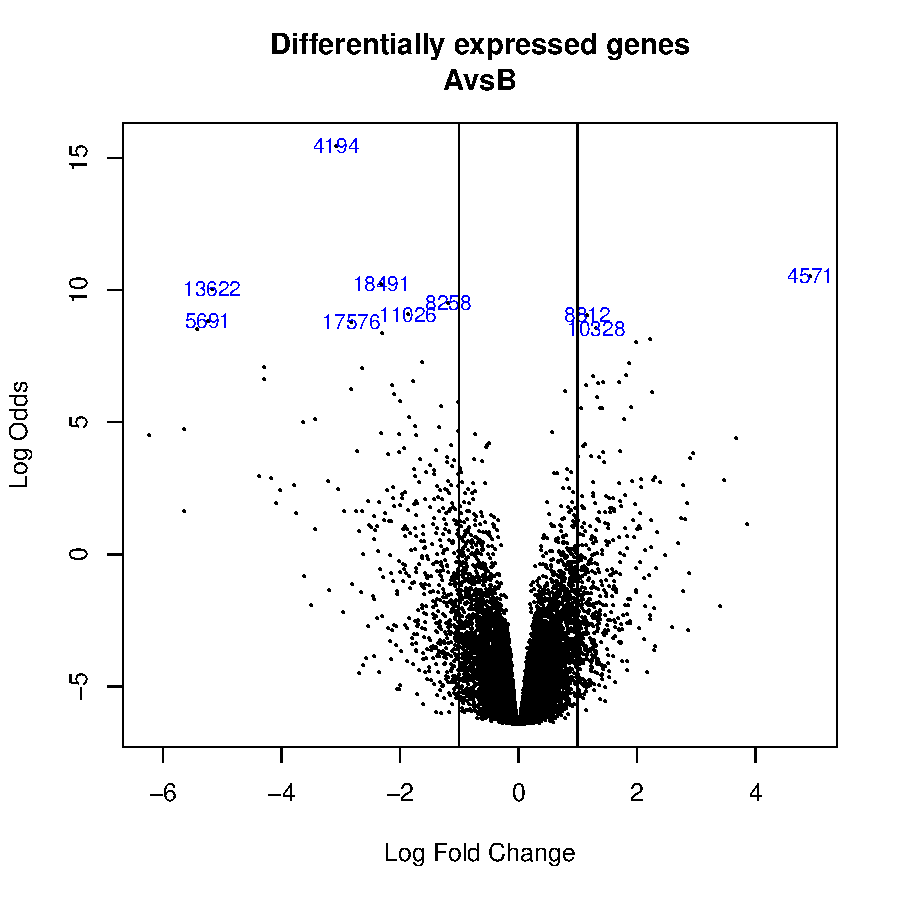
\includegraphics{volcanoPlotAvsB.pdf}

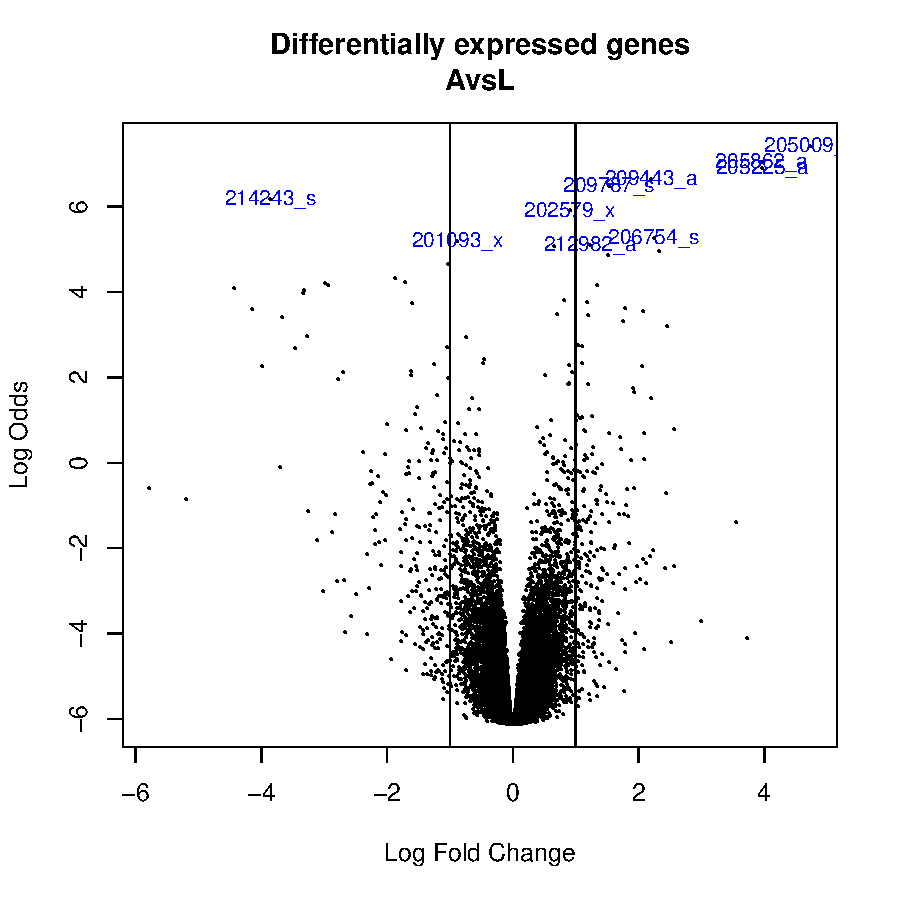
\includegraphics{volcanoPlotAvsL.pdf}

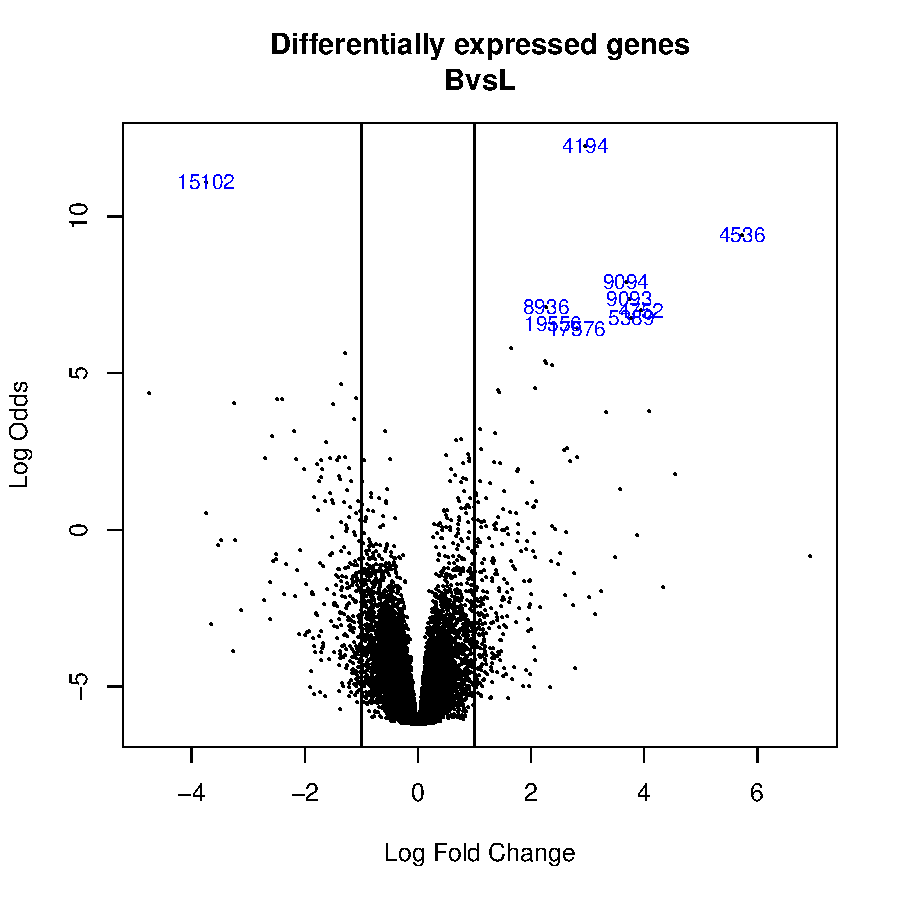
\includegraphics{volcanoPlotBvsL.pdf}



\subsubsection{Principales genes expresados diferencialmente}

Si consideráramos genes expresados diferencialmente aquellos que tienen un p--valor ajustado inferior a 0.05 o 0.01 el número de genes diferencialmente expresado en cada caso sería:

\begin{knitrout}
\definecolor{shadecolor}{rgb}{0.969, 0.969, 0.969}\color{fgcolor}\begin{kframe}
\begin{verbatim}
## Numero de genes con un p--valor inferior a 0.05 en cada comparación:
## En la comparación 'A vs B':  730
## En la comparación 'A vs L':  64
## En la comparación 'B vs L':  116
## 
## Numero de genes con un p--valor inferior a 0.01 en cada comparación:
## En la comparación 'A vs B':  165
## En la comparación 'A vs L':  32
## En la comparación 'B vs L':  28
\end{verbatim}
\end{kframe}
\end{knitrout}


Los 10 genes más expresados diferencialmente en cada comparación se muestran en las tablas siguientes:

\begin{kframe}


{\ttfamily\noindent\bfseries\color{errorcolor}{\#\# Error in `[.data.frame`(topTab\_AvsB, 1:10, 1:7): undefined columns selected}}

{\ttfamily\noindent\bfseries\color{errorcolor}{\#\# Error in print(AvsB10, tabular.environment = "{}longtable"{}, floating = FALSE): error in evaluating the argument 'x' in selecting a method for function 'print': Error: object 'AvsB10' not found}}\end{kframe}

\begin{kframe}


{\ttfamily\noindent\bfseries\color{errorcolor}{\#\# Error in `[.data.frame`(topTab\_AvsL, 1:10, 1:7): undefined columns selected}}

{\ttfamily\noindent\bfseries\color{errorcolor}{\#\# Error in print(AvsL10, tabular.environment = "{}longtable"{}, floating = FALSE): error in evaluating the argument 'x' in selecting a method for function 'print': Error: object 'AvsL10' not found}}\end{kframe}

\begin{kframe}


{\ttfamily\noindent\bfseries\color{errorcolor}{\#\# Error in `[.data.frame`(topTab\_BvsL, 1:10, 1:7): undefined columns selected}}

{\ttfamily\noindent\bfseries\color{errorcolor}{\#\# Error in print(BvsL10, tabular.environment = "{}longtable"{}, floating = FALSE): error in evaluating the argument 'x' in selecting a method for function 'print': Error: object 'BvsL10' not found}}\end{kframe}


\section{Post-procesado de las listas de genes obtenidas}

Una vez obtenidas las listas de genes diferencialmente expresados pueden llevarse a cabo todo tipo de análisis sobre ellas, generalmente encaminados a facilitar la interpretación de los resultados.

Entre estas exploraciones --que podemos llamar genericamente ``post-procesado de las listas'' se encuentra

\begin{itemize}
\item La anotación de las listas de genes en diversas bases de datos.

\item La comparación entre las listas para determinar que genes cambian simultaneamente -o no- en varias comparaciones (o cuales cambian en una comparación pero no en otra).
\item La visualización de todos los genes seleccionados en varias comparaciones para, de forma similar a lo anterior, detectar grupos de genes con patrones de cambio similares --o distintos-- entre distintas comparaciones.
\item EL análisis de significación biológica de las listas mediante análisis de enriquecimiento o mediante ``gene set analysis'' para detectar si las listas se encuentran enriquecidas en genes asociados a funciones o procesos biológicos determinados.
\end{itemize}


\subsection{Comparaciones múltiples}

Cuando se realizan varias comparaciones a la vez puede resultar importante ver 
que genes cambian simultáneamente en más de una comparación.
Si el número de comparaciones es alto también puede ser necesario realizar un 
ajuste de p-valores entre las comparaciones, distinto del realizado entre genes.

La función \texttt{decidetests} permite realizar ambas cosas.
En este ejemplo no se ajustaran los p--valores entre comparaciones. Tan solo se seleccionaran los genes que cambian en una o más condiciones.

EL resultado del análisis es una tabla \texttt{res} que para cada gen y cada comparación 
contiene un 1 (si el gen esta sobre-expresado o ``up'' en esta condicion), 
un 0 (si no hay cambio significativo) o un -1 
(si esta ``down''-regulado).



Para resumir dicho análisis podemos contar qué filas tienen como mínimo una celda distinta de cero:

\begin{knitrout}
\definecolor{shadecolor}{rgb}{0.969, 0.969, 0.969}\color{fgcolor}\begin{kframe}
\begin{alltt}
\hlstd{sum.res.rows}\hlkwb{<-}\hlkwd{apply}\hlstd{(}\hlkwd{abs}\hlstd{(res),}\hlnum{1}\hlstd{,sum)}
\hlstd{res.selected}\hlkwb{<-}\hlstd{res[sum.res.rows}\hlopt{!=}\hlnum{0}\hlstd{,]}
\hlkwd{print}\hlstd{(}\hlkwd{summary}\hlstd{(res))}
\end{alltt}
\begin{verbatim}
##     AvsB  AvsL  BvsL
## -1    67    12    10
## 0  22149 22256 22255
## 1     67    15    18
\end{verbatim}
\end{kframe}
\end{knitrout}

En vista de estos valores podemos aplicar otros criterios de selección, por ejemplo genes con un p-valor ajustado inferior a 0.05 y \texttt{log Fold change} mayor o igual a 1.\emph{ Este criterio combina a la vez la significación estadística y la significación biológica por lo que, en un estudio real sería probablemente el escogido}.

\begin{knitrout}
\definecolor{shadecolor}{rgb}{0.969, 0.969, 0.969}\color{fgcolor}\begin{kframe}
\begin{verbatim}
##     AvsB  AvsL  BvsL
## -1   197    24    39
## 0  21882 22235 22201
## 1    204    24    43
\end{verbatim}
\end{kframe}
\end{knitrout}

Un diagrama de Venn permite visualizar la tabla anterior sin diferenciar entre genes ``up'' o ``down'' regulados.

\begin{figure}
\begin{knitrout}
\definecolor{shadecolor}{rgb}{0.969, 0.969, 0.969}\color{fgcolor}\begin{kframe}
\begin{alltt}
\hlkwd{vennDiagram} \hlstd{(res.selected[,}\hlnum{1}\hlopt{:}\hlnum{3}\hlstd{],} \hlkwc{main}\hlstd{=}\hlstr{"Genes in common #1"}\hlstd{,} \hlkwc{cex}\hlstd{=}\hlnum{0.9}\hlstd{)}
\end{alltt}
\end{kframe}
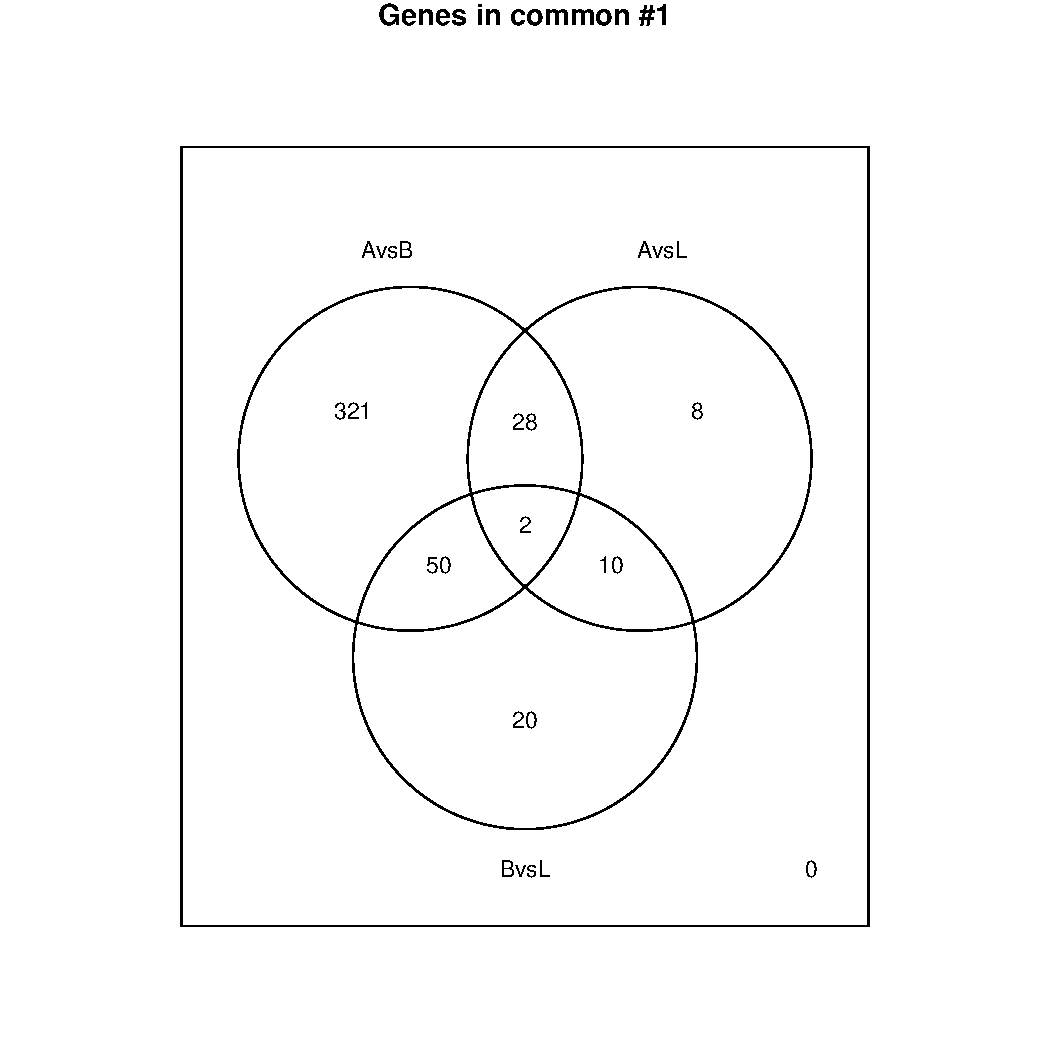
\includegraphics[width=\maxwidth]{images/graficvenn1-1} 

\end{knitrout}
\caption{\label{venn1}Número de genes seleccionado en cada comparación}
\end{figure}


\subsection{Anotación de resultados}

La identificación de los genes seleccionados puede resultar más sencilla para el especialista en un campo si se utilizan nombres estándar como el simbolo del gen o ``gene symbol''.
Con esta finalidad cada paquete de anotaciones tiene tablas de correspondencia entre los distintos tipos de identificadores, principalmente entre los del array y los de otras bases de datos.

Para saber que anotaciones estan disponibles debe cargarse el paquete y llamar la función del mismo nombre 

\begin{knitrout}
\definecolor{shadecolor}{rgb}{0.969, 0.969, 0.969}\color{fgcolor}\begin{kframe}
\begin{alltt}
\hlkwd{require}\hlstd{(hgu133a.db)}
\hlkwd{hgu133a}\hlstd{()}
\end{alltt}
\begin{verbatim}
## Quality control information for hgu133a:
## 
## 
## This package has the following mappings:
## 
## hgu133aACCNUM has 22283 mapped keys (of 22283 keys)
## hgu133aALIAS2PROBE has 45864 mapped keys (of 113648 keys)
\end{verbatim}


{\ttfamily\noindent\color{warningcolor}{\#\# Warning in (function () : hgu133aCHR is deprecated. Please use an appropriate TxDb object or\\\#\#\ \  package for this kind of data.}}\begin{verbatim}
## hgu133aCHR has 19843 mapped keys (of 22283 keys)
\end{verbatim}


{\ttfamily\noindent\color{warningcolor}{\#\# Warning in (function () : hgu133aCHRLENGTHS is deprecated. Please use an appropriate TxDb\\\#\#\ \  object or package for this kind of data.}}\begin{verbatim}
## hgu133aCHRLENGTHS has 93 mapped keys (of 93 keys)
\end{verbatim}


{\ttfamily\noindent\color{warningcolor}{\#\# Warning in (function () : hgu133aCHRLOC is deprecated. Please use an appropriate TxDb object\\\#\#\ \  or package for this kind of data.}}\begin{verbatim}
## hgu133aCHRLOC has 19639 mapped keys (of 22283 keys)
\end{verbatim}


{\ttfamily\noindent\color{warningcolor}{\#\# Warning in (function () : hgu133aCHRLOCEND is deprecated. Please use an appropriate TxDb\\\#\#\ \  object or package for this kind of data.}}\begin{verbatim}
## hgu133aCHRLOCEND has 19639 mapped keys (of 22283 keys)
## hgu133aENSEMBL has 19626 mapped keys (of 22283 keys)
## hgu133aENSEMBL2PROBE has 13664 mapped keys (of 28423 keys)
## hgu133aENTREZID has 19846 mapped keys (of 22283 keys)
## hgu133aENZYME has 3054 mapped keys (of 22283 keys)
## hgu133aENZYME2PROBE has 892 mapped keys (of 975 keys)
## hgu133aGENENAME has 19846 mapped keys (of 22283 keys)
## hgu133aGO has 19193 mapped keys (of 22283 keys)
## hgu133aGO2ALLPROBES has 18788 mapped keys (of 19541 keys)
## hgu133aGO2PROBE has 14415 mapped keys (of 15283 keys)
## hgu133aMAP has 19788 mapped keys (of 22283 keys)
## hgu133aOMIM has 17156 mapped keys (of 22283 keys)
## hgu133aPATH has 7873 mapped keys (of 22283 keys)
## hgu133aPATH2PROBE has 229 mapped keys (of 229 keys)
## hgu133aPMID has 19785 mapped keys (of 22283 keys)
## hgu133aPMID2PROBE has 416521 mapped keys (of 452385 keys)
## hgu133aREFSEQ has 19757 mapped keys (of 22283 keys)
## hgu133aSYMBOL has 19846 mapped keys (of 22283 keys)
## hgu133aUNIGENE has 19806 mapped keys (of 22283 keys)
## hgu133aUNIPROT has 19303 mapped keys (of 22283 keys)
## 
## 
## Additional Information about this package:
## 
## DB schema: HUMANCHIP_DB
## DB schema version: 2.1
## Organism: Homo sapiens
## Date for NCBI data: 2015-Mar17
## Date for GO data: 20150314
## Date for KEGG data: 2011-Mar15
## Date for Golden Path data: 2010-Mar22
## Date for Ensembl data: 2015-Mar13
\end{verbatim}
\end{kframe}
\end{knitrout}

Cada tabla de asociación puede consultarse de diversas formas, 
\begin{itemize}
\item Con las funciones \texttt{get} o \texttt{mget}.
\item Convirtiéndola en una tabla y extrayendo valores
\item En algunos casos utilizando funciones específicas como \texttt{getSYMBOL} o \texttt{getEG} (por ``Entrez Gene'') cuando exitan.
\end{itemize}

Bioconductor dispone de algunos paquetes que permiten aprovechar esta funcionalidad anterior para obtener las anotaciones de cada gen y generar una tabla HTML con enlaces a algunas bases de datos.

De forma sencilla es posible obtener tablas con las anotaciones correspondientes a los genes seleccionados. Si se desea ser más ambicioso es posible generar tablas en las que se combinen hiperenlaces a las anotaciones con los resultados de la selección de genes.

Veamos las distintas posibilidades, en orden de complejidad creciente

\subsubsection{Tablas de anotaciones sencillas}

El paquete \texttt{annafy} permite de forma muy simple generar una tabla de anotaciones con hiperenlaces a las bases de datos para cada anotación seleccionada.

La instrucción siguiente crea una tabla con las anotaciones disponibles para los genes seleccionados en la sección de comparaciones múltiples.

\begin{knitrout}
\definecolor{shadecolor}{rgb}{0.969, 0.969, 0.969}\color{fgcolor}\begin{kframe}
\begin{alltt}
\hlkwd{require}\hlstd{(annaffy)}
\hlstd{genesSelected} \hlkwb{<-} \hlkwd{rownames}\hlstd{(res.selected)}
\hlstd{at} \hlkwb{<-} \hlkwd{aafTableAnn}\hlstd{(genesSelected,} \hlstr{"hgu133a.db"}\hlstd{)}
\hlkwd{saveHTML} \hlstd{(at,} \hlkwd{file.path}\hlstd{(resultsDir,} \hlstr{"anotations.html"}\hlstd{),}
          \hlstr{"Annotations for selected genes"}\hlstd{)}
\end{alltt}
\end{kframe}
\end{knitrout}


\subsubsection{Archivos de resultados con tablas hiperenlazables}

La funcion \Rfun{htmlpage} permite generar un archivo html a partir de un \Rfun{data.frame} con una funcionalidad muy interesante: pdemos hacer que una o varias de sus columnas contengan hiperenlaces a alguna base de datos permitiendo acceder a gran cantidad de información sobre los genes de la lista.

Para aprender más sobre su uso se puede leer la viñeta \texttt{How to get pretty output} disponible en Bioconductor.

Mediante un bucle apropiado creamos una tabla anotada para cada comparación.

\begin{knitrout}
\definecolor{shadecolor}{rgb}{0.969, 0.969, 0.969}\color{fgcolor}\begin{kframe}
\begin{alltt}
\hlkwd{require}\hlstd{(annotate)}
\hlkwd{require}\hlstd{(hgu133a.db)}
\hlstd{listOfTables} \hlkwb{<-} \hlkwd{list}\hlstd{(}\hlkwc{AvsB} \hlstd{= topTab_AvsB,} \hlkwc{AvsL} \hlstd{= topTab_AvsL,} \hlkwc{BvsL} \hlstd{= topTab_BvsL)}
\hlkwa{for} \hlstd{(i} \hlkwa{in} \hlnum{1}\hlopt{:}\hlkwd{length}\hlstd{(listOfTables))\{}
  \hlcom{# Seleccionamos la "topTable"}
  \hlstd{topTab} \hlkwb{<-} \hlstd{listOfTables[[i]]}
  \hlcom{# Escogemos los grupos de sondas a incluir en la tabla}
  \hlstd{whichGenes}\hlkwb{<-}\hlstd{topTab[}\hlstr{"P.Value"}\hlstd{]}\hlopt{<}\hlnum{0.05}
  \hlstd{selectedIDs} \hlkwb{<-} \hlkwd{rownames}\hlstd{(topTab)[whichGenes]}
  \hlcom{# Los convertimos a identificadores Entrez ("EG") y a Gene Symbols}
  \hlstd{genes}\hlkwb{<-} \hlkwd{getEG}\hlstd{(selectedIDs,} \hlstr{"hgu133a.db"}\hlstd{)}
  \hlstd{simbols} \hlkwb{<-}\hlkwd{getSYMBOL}\hlstd{(selectedIDs,} \hlstr{"hgu133a.db"}\hlstd{)}
  \hlcom{# Haremos la columna de Entrez sea hiperenlazable}
  \hlstd{paraEnlace} \hlkwb{<-} \hlkwd{list} \hlstd{(}\hlkwc{misgenes}\hlstd{=genes)}
  \hlcom{# Preparamos el data.frame con el que se creará el archivo de resultados}
  \hlstd{otherNames} \hlkwb{=} \hlkwd{data.frame}\hlstd{(selectedIDs, simbols, topTab[whichGenes,}\hlopt{-}\hlnum{1}\hlstd{])}
  \hlkwd{names}\hlstd{(otherNames)} \hlkwb{=} \hlkwd{c}\hlstd{(}\hlstr{"Affy ID"}\hlstd{,} \hlstr{"Gene Symbol"}\hlstd{,} \hlkwd{colnames}\hlstd{(topTab)[}\hlopt{-}\hlnum{1}\hlstd{])}
  \hlcom{# Invocamos la función "htmlpage"}
  \hlstd{comparison} \hlkwb{<-} \hlkwd{names}\hlstd{(listOfTables)[i]}
  \hlkwd{htmlpage}\hlstd{(paraEnlace,}
           \hlkwc{filename} \hlstd{=}\hlkwd{file.path}\hlstd{(resultsDir,}
           \hlkwd{paste}\hlstd{(}\hlstr{"Selected Genes in comparison "}\hlstd{,comparison,}\hlstr{".html"}\hlstd{,} \hlkwc{sep}\hlstd{=}\hlstr{""}\hlstd{)) ,}
           \hlkwc{title} \hlstd{=} \hlkwd{paste}\hlstd{(}\hlstr{"Diff. expressed genes in comparison "}\hlstd{, comparison,} \hlkwc{sep}\hlstd{=}\hlstr{""}\hlstd{),}
           \hlkwc{othernames} \hlstd{= otherNames,}
           \hlkwc{table.head} \hlstd{=} \hlkwd{c}\hlstd{(}\hlstr{"Entrez IDs"}\hlstd{,} \hlkwd{names}\hlstd{(otherNames)),}
           \hlkwc{table.center} \hlstd{=} \hlnum{TRUE}\hlstd{,}
           \hlkwc{repository}\hlstd{=}\hlkwd{list}\hlstd{(}\hlstr{"en"}\hlstd{))}
\hlstd{\}}
\end{alltt}
\end{kframe}
\end{knitrout}

\subsection{Visualización de los perfiles de expresión}

Tras seleccionar los genes diferencialmente expresados podemos visualizar 
las expresiones de cada gen agrupándolas para destacar los genes que se 
encuentran up o down regulados simultáneamente constituyendo \emph{perfiles de expresión}.

Hay distintas formas de visualización pero aquí tan sólo se presenta el uso de mapas de color o 
\texttt{Heatmaps}.

En primer lugar seleccionamos los genes avisualizar: Se toman todos aquellos que 
han resultado diferencialmente expresados en alguna de las tres comparaciones.

\begin{knitrout}
\definecolor{shadecolor}{rgb}{0.969, 0.969, 0.969}\color{fgcolor}\begin{kframe}
\begin{alltt}
\hlstd{probeNames}\hlkwb{<-}\hlkwd{rownames}\hlstd{(res)}
\hlstd{probeNames.selected}\hlkwb{<-}\hlstd{probeNames[sum.res.rows}\hlopt{!=}\hlnum{0}\hlstd{]}
\hlstd{exprs2cluster} \hlkwb{<-}\hlkwd{exprs}\hlstd{(eset_rma)[probeNames.selected,]}
\hlkwd{colnames}\hlstd{(exprs2cluster)}\hlkwb{<-}\hlstd{sampleNames}
\hlstd{color.map} \hlkwb{<-} \hlkwa{function}\hlstd{(}\hlkwc{grupo}\hlstd{) \{}
  \hlkwa{if} \hlstd{(grupo}\hlopt{==}\hlstr{"A"}\hlstd{)\{}
    \hlstd{c}\hlkwb{<-} \hlstr{"yellow"}
  \hlstd{\}}\hlkwa{else}\hlstd{\{}
    \hlkwa{if} \hlstd{(grupo}\hlopt{==}\hlstr{"B"}\hlstd{)\{}
      \hlstd{c}\hlkwb{<-} \hlstr{"red"}
    \hlstd{\}}\hlkwa{else}\hlstd{\{}
      \hlstd{c}\hlkwb{<-} \hlstr{"blue"}
   \hlstd{\}}
  \hlstd{\}}
\hlkwd{return}\hlstd{(c)\}}
\end{alltt}
\end{kframe}
\end{knitrout}

Para representar el Heatmap tan sólo necesitamos la matriz de datos resultante.

\begin{figure}[htbp]
\centering
\begin{knitrout}
\definecolor{shadecolor}{rgb}{0.969, 0.969, 0.969}\color{fgcolor}\begin{kframe}
\begin{alltt}
\hlstd{grupColors} \hlkwb{<-} \hlkwd{unlist}\hlstd{(}\hlkwd{lapply}\hlstd{(}\hlkwd{pData}\hlstd{(eset_rma)}\hlopt{$}\hlstd{Group, color.map))}
\hlkwd{heatmap}\hlstd{(exprs2cluster,} \hlkwc{col}\hlstd{=}\hlkwd{rainbow}\hlstd{(}\hlnum{100}\hlstd{),} \hlkwc{ColSideColors}\hlstd{=grupColors,} \hlkwc{cexCol}\hlstd{=}\hlnum{0.9}\hlstd{)}
\end{alltt}
\end{kframe}
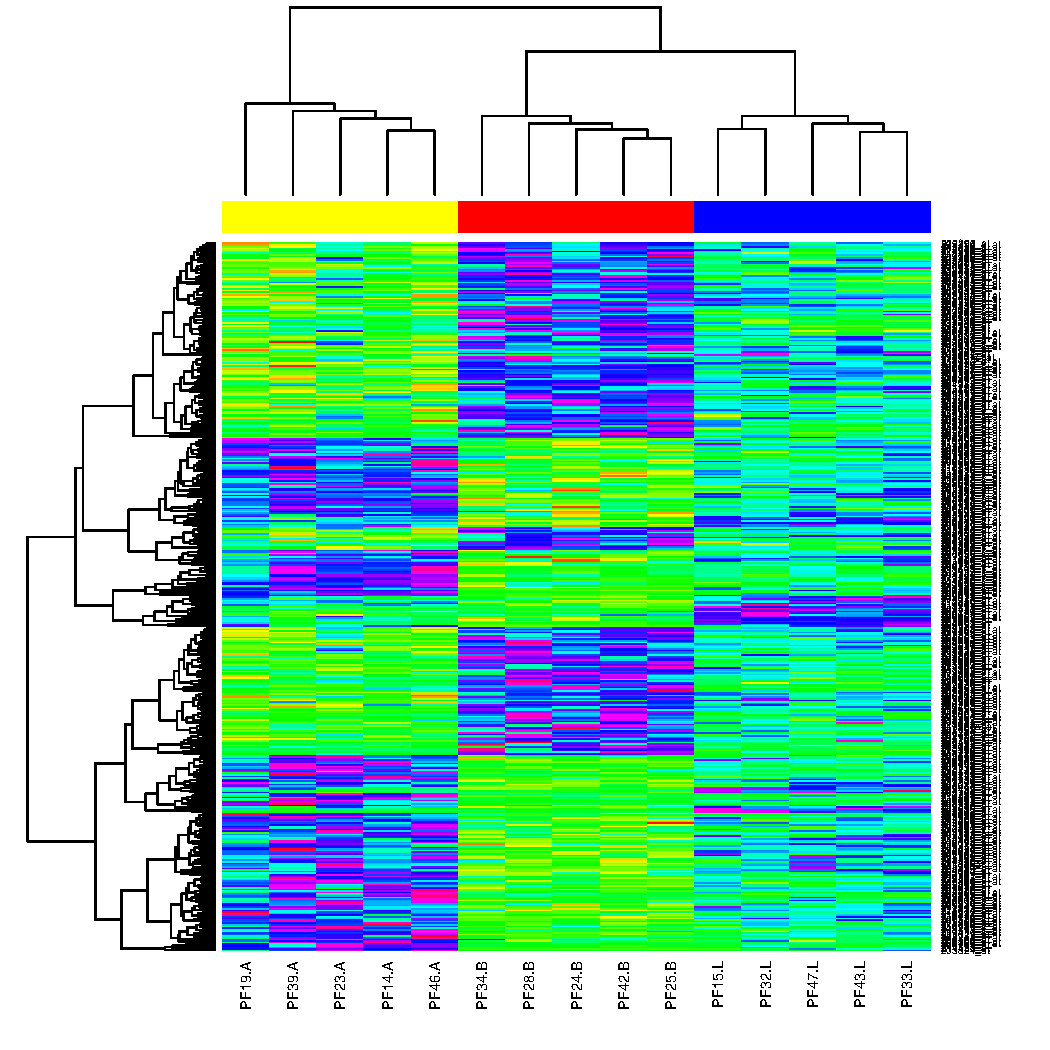
\includegraphics[width=\maxwidth]{images/graficplotHeatMap1-1} 

\end{knitrout}
\caption{Mapa de colores basado en los genes seleccionados por estar diferencialmente expresados. Como puede verse los tumores Apocrinos y Luminales tienen perfiles de expresión más parecidos entre ellos que cada uno con los de tipo Basal}
\label{fig:heatmap1}
\end{figure}

Si se desea realizar mapas de color más sofisticados puede utilizarse el paquete \Rpackage{gplots}
que implementa una version mejorada en la función \texttt{heatmap.2}


\begin{figure}[htbp]
\centering
\begin{knitrout}
\definecolor{shadecolor}{rgb}{0.969, 0.969, 0.969}\color{fgcolor}\begin{kframe}
\begin{alltt}
\hlstd{grupColors} \hlkwb{<-} \hlkwd{unlist}\hlstd{(}\hlkwd{lapply}\hlstd{(}\hlkwd{pData}\hlstd{(eset_rma)}\hlopt{$}\hlstd{Group, color.map))}
\hlkwd{require}\hlstd{(}\hlstr{"gplots"}\hlstd{)}
\hlkwd{heatmap.2}\hlstd{(exprs2cluster,}
          \hlkwc{col}\hlstd{=}\hlkwd{bluered}\hlstd{(}\hlnum{75}\hlstd{),} \hlkwc{scale}\hlstd{=}\hlstr{"row"}\hlstd{,}
          \hlkwc{ColSideColors}\hlstd{=grupColors,} \hlkwc{key}\hlstd{=}\hlnum{TRUE}\hlstd{,} \hlkwc{symkey}\hlstd{=}\hlnum{FALSE}\hlstd{,}
          \hlkwc{density.info}\hlstd{=}\hlstr{"none"}\hlstd{,} \hlkwc{trace}\hlstd{=}\hlstr{"none"}\hlstd{,} \hlkwc{cexCol}\hlstd{=}\hlnum{1}\hlstd{)}
\end{alltt}
\end{kframe}
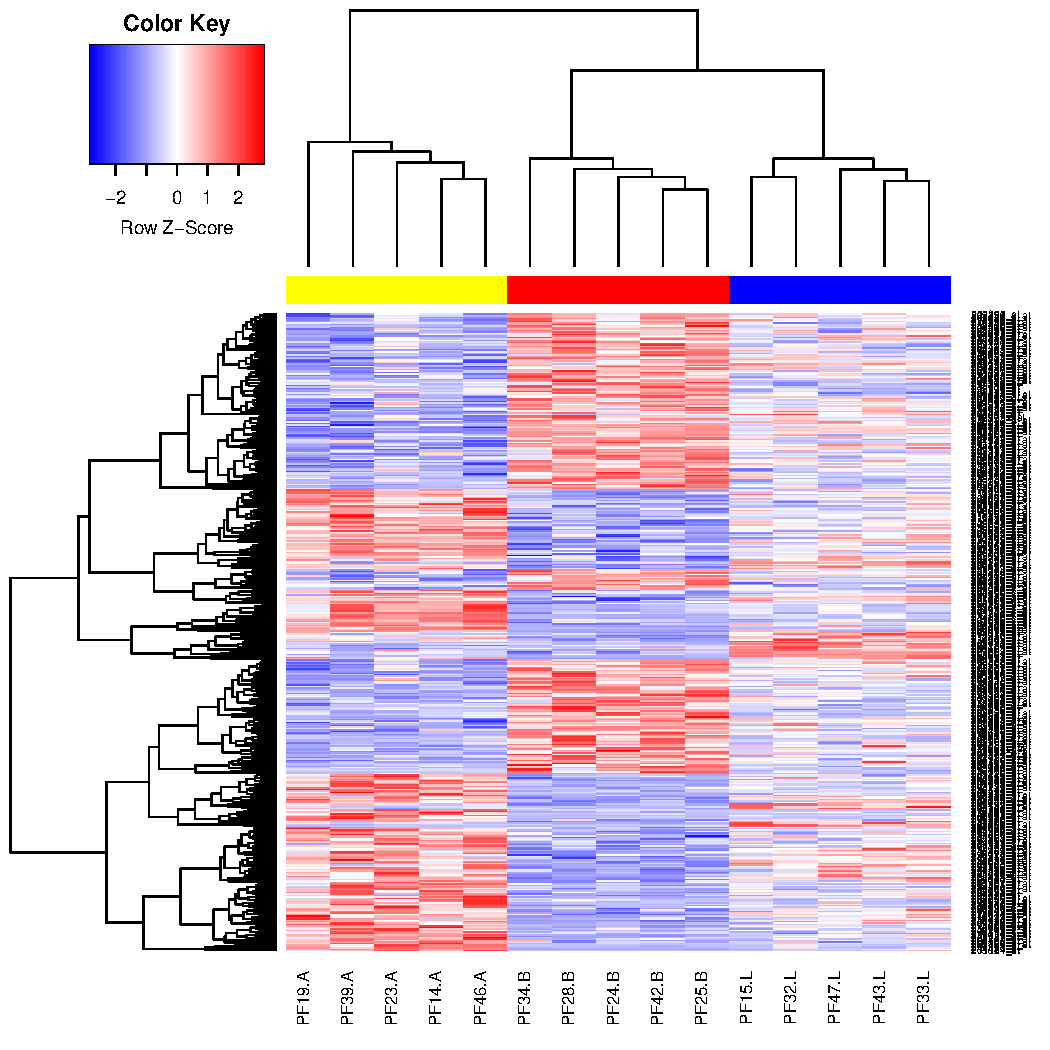
\includegraphics[width=\maxwidth]{images/graficplotHeatMap2-1} 

\end{knitrout}
\caption{Mapa de colores mejorado basado en los genes seleccionados por estar diferencialmente expresados. Como puede verse los tumores Apocrinos y Luminales tienen perfiles de expresión más parecidos entre ellos que cada uno con los de tipo Basal}
\label{fig:heatmap2}
\end{figure}



\subsection{Análisis de la significación biológica}

El análisis de significación biológica busca establecer si, dada una lista de genes seleccionados por estar diferencialmente expresados entre dos condiciones, las funciones y procesos biológicos que los caracterizan aparecen en esta lista con mayor frecuencia que entre el resto de genes analizados.

Se han desarrollad multitud de variantes de estos tipos de análisis (\cite{Khatri:2005}) pero aquí utilizaremos el análisis básico de enriquecimiento tal como se describe en los trabajos de Gentleman (\cite{Gentleman:2004}) implementados en el paquete \texttt{GOstats} de Bioconductor.

El análisis se realiza sobre dos bases de datos de anotaciones, la "Gene Ontology'' o la ``Kyoto Encyclopedia of Genes and Genomes''.

Los análisis de este tipo necesitan un número mínimo de genes para resultar fiables por lo que se incluiran en todos los genes con p--valores ajustados inferiores a 0.05 (sin filtrar por minimo ``fold--change'').

\begin{knitrout}
\definecolor{shadecolor}{rgb}{0.969, 0.969, 0.969}\color{fgcolor}\begin{kframe}
\begin{alltt}
\hlkwd{require}\hlstd{(GOstats)}
\hlstd{listOfTables} \hlkwb{<-} \hlkwd{list}\hlstd{(}\hlkwc{AvsB} \hlstd{= topTab_AvsB,} \hlkwc{AvsL} \hlstd{= topTab_AvsL,} \hlkwc{BvsL} \hlstd{= topTab_BvsL)}
\hlkwa{for} \hlstd{(i} \hlkwa{in} \hlnum{1}\hlopt{:}\hlkwd{length}\hlstd{(listOfTables))\{}
  \hlcom{# Seleccionamos la "topTable"}
  \hlstd{topTab} \hlkwb{<-} \hlstd{listOfTables[[i]]}
  \hlcom{# Definimos el universo de genes: todos los que se han incluido en el análisis}
  \hlcom{# EL programa trabaja con identificadores "entrez" y no admite duplicados}

  \hlstd{entrezUniverse} \hlkwb{=} \hlkwd{unique}\hlstd{(}\hlkwd{getEG}\hlstd{(}\hlkwd{as.character}\hlstd{(topTab}\hlopt{$}\hlstd{ID),} \hlstr{"hgu133a.db"}\hlstd{))}

  \hlcom{# Escogemos los grupos de sondas a incluir en el análisis}
  \hlcom{# Este análisis trabaja bien con varios centenares de genes }
  \hlcom{# por lo que es habitual basarse en p-valores sin ajustar para incluirlos}

  \hlstd{whichGenes}\hlkwb{<-}\hlstd{topTab[}\hlstr{"adj.P.Val"}\hlstd{]}\hlopt{<}\hlnum{0.05}
  \hlstd{geneIds} \hlkwb{<-}   \hlkwd{unique}\hlstd{(}\hlkwd{getEG}\hlstd{(}\hlkwd{as.character}\hlstd{(topTab}\hlopt{$}\hlstd{ID[whichGenes]),}\hlstr{"hgu133a.db"}\hlstd{))}

  \hlcom{# Creamos los "hiperparámetros" en que se basa el análisis}
  \hlstd{GOparams} \hlkwb{=} \hlkwd{new}\hlstd{(}\hlstr{"GOHyperGParams"}\hlstd{,}
    \hlkwc{geneIds}\hlstd{=geneIds,} \hlkwc{universeGeneIds}\hlstd{=entrezUniverse,}
    \hlkwc{annotation}\hlstd{=}\hlstr{"org.Hs.eg.db"}\hlstd{,} \hlkwc{ontology}\hlstd{=}\hlstr{"BP"}\hlstd{,}
    \hlkwc{pvalueCutoff}\hlstd{=}\hlnum{0.001}\hlstd{,} \hlkwc{conditional}\hlstd{=}\hlnum{FALSE}\hlstd{,}
    \hlkwc{testDirection}\hlstd{=}\hlstr{"over"}\hlstd{)}
  \hlstd{KEGGparams} \hlkwb{=} \hlkwd{new}\hlstd{(}\hlstr{"KEGGHyperGParams"}\hlstd{,}
    \hlkwc{geneIds}\hlstd{=geneIds,} \hlkwc{universeGeneIds}\hlstd{=entrezUniverse,}
    \hlkwc{annotation}\hlstd{=}\hlstr{"org.Hs.eg.db"}\hlstd{,}
    \hlkwc{pvalueCutoff}\hlstd{=}\hlnum{0.01}\hlstd{,} \hlkwc{testDirection}\hlstd{=}\hlstr{"over"}\hlstd{)}

  \hlcom{# Ejecutamos los análisis}

  \hlstd{GOhyper} \hlkwb{=} \hlkwd{hyperGTest}\hlstd{(GOparams)}
  \hlstd{KEGGhyper} \hlkwb{=} \hlkwd{hyperGTest}\hlstd{(KEGGparams)}

\hlcom{# Creamos un informe html con los resultados}
   \hlstd{comparison} \hlkwb{=} \hlkwd{names}\hlstd{(listOfTables)[i]}
   \hlstd{GOfilename} \hlkwb{=}\hlkwd{file.path}\hlstd{(resultsDir,}
     \hlkwd{paste}\hlstd{(}\hlstr{"GOResults."}\hlstd{,comparison,}\hlstr{".html"}\hlstd{,} \hlkwc{sep}\hlstd{=}\hlstr{""}\hlstd{))}
   \hlstd{KEGGfilename} \hlkwb{=}\hlkwd{file.path}\hlstd{(resultsDir,}
     \hlkwd{paste}\hlstd{(}\hlstr{"KEGGResults."}\hlstd{,comparison,}\hlstr{".html"}\hlstd{,} \hlkwc{sep}\hlstd{=}\hlstr{""}\hlstd{))}
  \hlkwd{htmlReport}\hlstd{(GOhyper,} \hlkwc{file} \hlstd{= GOfilename,} \hlkwc{summary.args}\hlstd{=}\hlkwd{list}\hlstd{(}\hlstr{"htmlLinks"}\hlstd{=}\hlnum{TRUE}\hlstd{))}
  \hlkwd{htmlReport}\hlstd{(KEGGhyper,} \hlkwc{file} \hlstd{= KEGGfilename,} \hlkwc{summary.args}\hlstd{=}\hlkwd{list}\hlstd{(}\hlstr{"htmlLinks"}\hlstd{=}\hlnum{TRUE}\hlstd{))}
\hlstd{\}}
\end{alltt}


{\ttfamily\noindent\bfseries\color{errorcolor}{\#\# Error in unique(getEG(as.character(topTab\$ID), "{}hgu133a.db"{})): error in evaluating the argument 'x' in selecting a method for function 'unique': Error in unlist(lookUp(x, data, "{}ENTREZID"{})) : \\\#\#\ \  error in evaluating the argument 'x' in selecting a method for function 'unlist': Error in lookUp(x, data, "{}ENTREZID"{}) : No keys provided\\\#\# Calls: getEG -> unlist}}\end{kframe}
\end{knitrout}

\section{Resumen de resultados y discusión}

Los controles de calidad llevados a cabo en la primera parte de  este estudio han permitido establecer que los datos con los que se ha trabajado eran de buena calidad, a pesar de presentar una cierta heterogeneidad que queda ilustrada en la incompleta agrupación de las muestras segun sus tipos de tumores.

Los análisis llevados a cabo sobre los datos normalizados y filtrados han permitido detectar un cierto número de genes diferencialmente expresados (ver tabla \ref{resum1}) que se prestan a estudios posteriores acerca de su significación biológica.

\begin{table}[htbp]
\caption{Genes diferencialmente expresados basados en un cirte definido por un p-valor ajustado (FDR) inferior a 0.05 y un cambio de expresión de cómo mínimo 1.}
\begin{tabular}{|l|c|c|c|}
\hline
 & A vs B & A vs L & B vs L \\ \hline
Genes “down-regulados” & 228 & 29 & 113 \\ \hline
Genes “sobre-expresados” & 174 & 27 & 111 \\ \hline
\end{tabular}
\label{resum1}
\end{table}

La lista completas de genes seleccionados (ordenados de mayor a menor p--valor) pueden verse en los archivos ``Selected genes in comparison AvsB.html'', ``Selected genes in comparison AvsL.html'' y ``Selected genes in comparison BvsL.html''.

El análisis de significación biológica ha permitido detectar una serie de funciones y procesos biológicos que caracterizan las listas de genes seleccionadas en las bases de datos de anotaciones más populares, la Gene Ontology (GO) y la ``Kyoto Enyclopedia of Genes and Genomes''. Estas listas pueden verse en las tablas ``GOResults.XXvsYY.html'' y ``KEGGResults.XXvsYY.html'' (XXvsYY es AvsB, AvsL o BvsL) pero no se discuten aquí.

\subsection{Discusión}

El estudio que se ha presentado en este documento es un análisis estándar de microarrays y como tal adolece de sus ventajas e inconvenientes.

Como inconveniente podemos destacar dos cosas
\begin{itemize}
\item El tamaño de las muestras utilizadas es bastante limitado lo que determina que el estudio tenga poca potencia por lo que \emph{probablemente} habrá menos reproducibilidad y más falsos negativos de los que sería deseable si se utilizara un mayor número de muestras.
\item En cada paso del proceso se han tomado decisiones relativamente arbitrarias acerca de los métodos a seguir para la normalización, filtradom selección de genes, etc. La decisión de si estos métodos son los más adecuados o no es probablemente subjetiva (véase por ejemplo los artículos ~\cite{Choe:2005, Zhu:2010}) por lo que sería interesante saber como cambian los resultados si se tomaran otras decisiones.
\end{itemize}

Los problemas anteriores no son, sin embargo, problemas de este estudio concreto, sino en general de los estudios basados en microarrays por lo que, limitaciones aparte, el estudio aportará probablemente información valiosa que permitirá un seguimiento posterior del problema.

Finalmente debe de tenerse en cuenta que cualquier gen que se acabe considerando realmente expresado diferencialmente se tendrá que verificar mediante otras técnicas como RT-qPCR por lo que este estudio debe de considerarse como un paso hacia el descubrimiento de genes candidatos, no como una fase definitiva.


%\subsubsection{Tablas de resultados}
%Un análisis como el que se ha realizado en este ejercicio genera una gran cantidad de archivos de resultados. \emph{Una buena práctica} en estos casos es preparar algun tipo de tabla que permita tener una visión panorámica de los resultados o navegar entre ellos.
%Esto puede hacers de forma relativamente sencilla con el paquete \texttt{hwriter}

\bibliography{MDA-references}

\appendix{Codigo R del análisis}

El archivo \texttt{Solucion_PEC_Microarrays.R} contiene el código R utilizado para realizar todos los análisis presentados en este informe.

El análisis se ha llevado a cabo utilizando el sistema \texttt{Sweave} (\cite{Leisch:2002a, Leisch:2002b}) de análisis reproducibles que integra el sistema \LaTeX y el lenguaje \R para generar a la vez los análisis y el informe de resultados por lo que el código puede contener alguna instrucción inusual cuando su objetivo es generar una tabla de \LaTeX. Aparte de ésto es un código estándar en el que se ha procurado no usar funciones avanzadas sino básicamente lo que se ha discutido en el curso.

\appendix{Lista de archivos generados en el estudio}

La tabla \ref{listaArchivos} contiene una lista de los archivos generados en este estudio. 

\begin{kframe}


{\ttfamily\noindent\itshape\color{messagecolor}{\#\# Loading required package: gdata\\\#\# gdata: read.xls support for 'XLS' (Excel 97-2004) files ENABLED.\\\#\# \\\#\# gdata: read.xls support for 'XLSX' (Excel 2007+) files ENABLED.\\\#\# \\\#\# Attaching package: 'gdata'\\\#\# \\\#\# The following object is masked from 'package:IRanges':\\\#\# \\\#\#\ \ \ \  trim\\\#\# \\\#\# The following object is masked from 'package:stats4':\\\#\# \\\#\#\ \ \ \  nobs\\\#\# \\\#\# The following object is masked from 'package:Biobase':\\\#\# \\\#\#\ \ \ \  combine\\\#\# \\\#\# The following object is masked from 'package:BiocGenerics':\\\#\# \\\#\#\ \ \ \  combine\\\#\# \\\#\# The following object is masked from 'package:stats':\\\#\# \\\#\#\ \ \ \  nobs\\\#\# \\\#\# The following object is masked from 'package:utils':\\\#\# \\\#\#\ \ \ \  object.size}}

{\ttfamily\noindent\color{warningcolor}{\#\# Warning in file(file, "{}rt"{}): cannot open file '/home/alex/Dropbox (VHIR)/Scripts/Exemple\_Analisis\_BioC/results/listaArchivos.txt': El fitxer o directori no existeix}}

{\ttfamily\noindent\bfseries\color{errorcolor}{\#\# Error in file(file, "{}rt"{}): cannot open the connection}}

{\ttfamily\noindent\bfseries\color{errorcolor}{\#\# Error in xtable(listaArchivos, label = "{}listaArchivos"{}, caption = "{}Lista de archivos generados en este análisis"{}): object 'listaArchivos' not found}}\end{kframe}% latex table generated in R 3.2.2 by xtable 1.7-4 package
% Sun Jan 10 17:26:00 2016
\begin{longtable}{rllll}
  \hline
 & Sample & Ids & SampleIDs & Group \\ 
  \hline
GSM26878.CEL & GSM26878 & PF14 EnPnT2N1G2 & PF14 & A \\ 
  GSM26883.CEL & GSM26883 & PF19 EnPuT4N0Gu & PF19 & A \\ 
  GSM26887.CEL & GSM26887 & PF23 EnPnT2N0G2 & PF23 & A \\ 
  GSM26903.CEL & GSM26903 & PF39 EnPuT4N0Gu & PF39 & A \\ 
  GSM26910.CEL & GSM26910 & PF46 EnPnT4N1G3 & PF46 & A \\ 
  GSM26888.CEL & GSM26888 & PF24 EnPnTiN0G3 & PF24 & B \\ 
  GSM26889.CEL & GSM26889 & PF25 EnPnT3N2G2 & PF25 & B \\ 
  GSM26892.CEL & GSM26892 & PF28 EnPnT2N1G3 & PF28 & B \\ 
  GSM26898.CEL & GSM26898 & PF34 EnPnT3N1G3 & PF34 & B \\ 
  GSM26906.CEL & GSM26906 & PF42 EnPnT2N2G3 & PF42 & B \\ 
  GSM26879.CEL & GSM26879 & PF15 EpPnTiN1G3 & PF15 & L \\ 
  GSM26896.CEL & GSM26896 & PF32 EpPnT3N1G2 & PF32 & L \\ 
  GSM26897.CEL & GSM26897 & PF33 EpPnTiN0G2 & PF33 & L \\ 
  GSM26907.CEL & GSM26907 & PF43 EpPpT2N1G2 & PF43 & L \\ 
  GSM26911.CEL & GSM26911 & PF47 EpPpT3N1G3 & PF47 & L \\ 
   \hline
\hline
\caption{Archivo targets.txt con la asignación a cada muestra de su condición experimental} 
\label{table.targets}
\end{longtable}


Utilizando el paquete \texttt{hwriter} es posible generar de forma sencilla una tabla html con hiperenlaces que permita acceder a los distintos archivos generados en el análisis.

\begin{knitrout}
\definecolor{shadecolor}{rgb}{0.969, 0.969, 0.969}\color{fgcolor}\begin{kframe}


{\ttfamily\noindent\bfseries\color{errorcolor}{\#\# Error in hwrite(listaArchivos, file.path(resultsDir, "{}listaArchivos.html"{})): object 'listaArchivos' not found}}\end{kframe}
\end{knitrout}



\end{document}
